\documentclass[12pt,oneside,reqno,english]{amsart}
\linespread{1.3}
%\usepackage[T1]{fontenc}
%\usepackage[latin9]{inputenc}
\pagestyle{plain}
\usepackage[left=1in,right=1in,top=1in, bottom=1in]{geometry}
\pagestyle{plain}
\usepackage{float}
\usepackage{amsthm}
\usepackage{amssymb}
\usepackage{natbib}
\usepackage{enumitem}
\usepackage{amsmath}
\usepackage{graphicx}
\usepackage{float}
\usepackage{graphicx}
\usepackage{setspace}
\setstretch{2}
\usepackage[leqno]{amsmath}
\usepackage{color}
\usepackage{tikz-cd}
\usepackage[hang,small,bf]{caption}
\usepackage[subrefformat=parens]{subcaption}
\captionsetup{compatibility=false}
\usetikzlibrary{decorations.pathmorphing}
\usepackage{chngcntr}
\usepackage{apptools}
\AtAppendix{\counterwithin{lemma}{section}}
\AtAppendix{\counterwithin{corollary}{section}}
\makeatletter
\renewcommand\subsection{\@startsection{subsection}{2}%
  \z@{-.5\linespacing\@plus-.7\linespacing}{.5\linespacing}%
  {\normalfont\scshape}}
\renewcommand\subsubsection{\@startsection{subsubsection}{3}%
  \z@{.5\linespacing\@plus.7\linespacing}{-.5em}%
  {\normalfont\scshape}}

\newcommand{\reqnomode}{\tagsleft@false}
\renewcommand{\baselinestretch}{1.3}
\newcommand{\lleft }{\left\{ }
\newcommand{\rright }{\right\} }
\def\R{\mathbb R}
\def\sumn{\sum_{i=1}^{n}}

\theoremstyle{definition}
\makeatother
\newtheorem{theorem}{Theorem}
\newtheorem{corollary}{Corollary}
\newtheorem{lemma}{Lemma}

\newtheorem*{thmC}{Convolution Theorem}
\newtheorem*{thmLP}{Theorem (Fang and Santos)}
\newtheorem*{thm1}{Theorem 1}
\newtheorem*{thm2}{Theorem 2}
\newtheorem*{thm3}{Theorem 3}
\newtheorem*{prop1}{Proposition 4}
\newtheorem*{prop2}{Proposition 2}

\newtheorem*{thmW}{Theorem (Weak convergence)}
\newtheorem*{thmB}{Theorem (Bootstrap consistency)}
\newtheorem*{cex}{Counter Example}
\newtheorem*{ex1}{Example 1}
\newtheorem*{ex2}{Example 2}
\newtheorem*{ex3}{Example 3}
\newtheorem*{ex4}{Example 4}

\newtheorem*{defH}{Definition (Hadamard directionally differentiable)}
\newtheorem*{asmN}{Assumption N}
\newtheorem*{asmD}{Assumption D}
\newtheorem*{asmG}{Assumption G}
\newtheorem*{asmB}{Assumption B}
\newtheorem*{lem1}{Lemma 1}
\newtheorem*{lem2}{Lemma 2}
\newtheorem*{lem3}{Lemma 3}
\newtheorem*{defP}{Definition (Pseudometric on $\mathcal{G}$)}

\usepackage{babel}

\makeatother
\begin{document}
\bibliographystyle{chicago}
\reqnomode

\title{Statistical Inference for Treatment Assignment Policies} 

\author{Yoshiyasu Rai}

\address{Department of Economics, University of Wisconsin-Madison, 1180 Observatory
Drive, Madison, WI 53706, USA.}

\email{yrai@wisc.edu}

\begin{abstract}
In this paper, I study the statistical inference problem for treatment assignment policies. In typical applications, individuals with different characteristics are expected to differ in their responses to treatment. Hence, treatment assignment policies that allocate treatment based on individuals' observed characteristics can have a significant influence on outcomes and welfare. 
A growing literature proposes various approaches to estimating the welfare-maximizing treatment assignment policy. I develop a method for assessing the precision of estimated optimal policies. In particular, for the welfare criterion used by \cite{KT:18} to propose estimated assignment policy, my method constructs (i) a confidence set for the optimal policy and (ii) a confidence interval for the maximized welfare. A simulation study indicates that the proposed methods work reasonably well with modest sample size. I apply the method to experimental data from the National Job Training Partnership Act study.
\end{abstract}
\maketitle

\section{Introduction}
Individuals with different characteristics often differ in their responses to treatment. 
As a result, treatment assignment policies that allocate treatment based on individuals' observed characteristics can have a significant influence on outcomes and welfare. 
This motivates methods that estimate treatment assignment policies that achieve high overall welfare. 
 Inspired by \cite{Manski:04}, there are a large number of existing studies on developing treatment assignment rules in econometrics 
 \citep{Dehejia:05, Stoye:09, Stoye:12, HP:09, Chamberlain:11, BD:12,Tetenov:12, Kasy:14,Kasy:16,KT:17, KT:18,MT:16, AW:17, MT:18}.
Measuring the performance of an existing assignment policy or quantifying the welfare impact of the optimal assignment policy 
can also provide useful information for a policymaker. 
In this paper, I contribute to the literature by proposing statistical inference methods for the treatment assignment policy to answer these questions. 

The first method I propose is a confidence set for the optimal assignment policy. 
The confidence set contains the optimal assignment policy that maximizes the mean outcome among all feasible policies with a prespecified level.
The set is constructed from test inversion, where for each feasible assignment policy, I implement a test for whether the assignment policy 
achieves the highest average outcome. The proposed confidence set is then defined as the collection of policies that are not rejected by the test. 
This method can also be used to test if any given assignment policy such as the current assignment policy or the policy that the policymaker proposes based on his/her knowledge can be rationalized as the average outcome maximizing policy. The second method is a confidence interval for the average outcome under the feasible optimal policy. This confidence interval quantifies what the researcher can learn from the data concerning the impact of the optimal policy on the average outcome. 


These inference methods build on two new results detailed in section \ref{main}. 
The first result considers welfare or the average outcome estimator.
I treat the average outcome estimator as an empirical process on the possibly infinite-dimensional treatment assignment policy space. I derive the asymptotic 
properties of this process. My results extend the asymptotic normality result for the average treatment effect estimator to the average outcome function estimator by showing that the estimator weakly converges to a Gaussian process uniformly over data distribution. This uniform convergence result is critical to allow test inversion to yield confidence sets for the optimal treatment assignment policy or the corresponding welfare measure. The estimator also accommodates both unknown propensity score and known propensity score cases. I then propose a bootstrap estimator that consistently approximates the limiting process. 
Second, I propose asymptotically valid tests to construct confidence sets based on the average outcome estimator and the bootstrap. 
As the parameter of interest involves a maximum of the average outcome, asymptotic inference is non-standard due to the potential non-differentiability \citep{HP:12}. 
To establish asymptotically valid inference results, I apply the 
inference method for possibly non-differentiable functionals recently studied in \cite{FS:16} and \cite{HL:18}. 
Their results can be used to show the test is consistent and nonconservative under fixed data distributions. 
The new finding in section \ref{main} shows that this test achieves uniform size control over a class of data distributions. This uniformity property is critical to the validity of the corresponding confidence sets.   

\subsection{Related literature}

There is a growing literature on treatment assignment rules in econometrics including 
\cite{Manski:04}, \cite{Dehejia:05}, \cite{Stoye:09,Stoye:12}, \cite{HP:09},\cite{Chamberlain:11}, \cite{BD:12}, \cite{Tetenov:12}, \cite{Kasy:14,Kasy:16}, \cite{KT:17,KT:18}, \cite{MT:16}, \cite{AW:17}
and \cite{MT:18}.
For discrete covariates, \cite{Manski:04} formalizes the treatment choice problem as an application of statistical decision theory and
proposes a Conditional Empirical Success (CES) rule that maximizes a sample analog of the welfare function.
\cite{Stoye:09} extends \cite{Manski:04} by showing the exact minmax decision rule. \cite{HP:09} propose a regression-based assignment rule and show its asymptotic optimality by utilizing the limit normal experiment.  

When there is a restriction on feasible assignment policies, 
\cite{KT:18} propose Empirical Welfare Maximization (EWM) that generalizes CES.   
They first estimate the average outcome function (empirical welfare) from the data and then select a maximizer from a restricted class of policies as a treatment assignment rule. They show the optimality of EWM in the sense that the method achieves the minmax regret rate bound. \cite{MT:16} extend EWM and propose the Penalized Welfare Maximization rule. 
While \cite{KT:18} focus on the rule that maximizes the inverse propensity score weighted estimate of the average outcome function, 
\cite{DLL:11} and \cite{AW:17} propose a rule that maximizes the doubly robust estimate. 
In \cite{AW:17}, they show that the rule based on the semiparametrically efficient average outcome estimator leads to a tighter regret upper bound.
Other rules based on empirical welfare function maximization are proposed by \cite{ZZRK:12} and 
\cite{ZMKK:17}.
In this paper, I follow the setting in \cite{KT:18} and \cite{AW:17} and consider 
maximizing an average outcome measure of welfare over a restricted class of feasible policies.

Statistical inference on treatment assignment policies has gained less attention than the estimation problem, but there are some notable exceptions.  
\cite{AS:14} consider an inference problem for the set of individuals who should be treated under the optimal assignment policy. 
By applying a multiple hypothesis testing method, they propose a random set of individual characteristics for which the data exhibit strong evidence of a positive conditional average treatment effect. 
\cite{BD:12} and \cite{LV:16} study inference for the maximum average outcome. 
Their result however, does not apply to my setting as I consider the exogenously restricted class of feasible policies. 
\cite{AKM:18} also consider inference on the average outcome. 
In their paper, they consider a general conditional inference problem for the estimated parameter that is selected from the data as a maximizer of some criterion.   
They then apply the method to the EWM problem. Their method provides valid inference on the average outcome that would realize if the policy selected from EWM were implemented. While \cite{AKM:18} provide inference for an \textit{estimated} optimal rule, my approach provides inference for the optimal rule itself. Also, \cite{AKM:18} provide a conditional inference method that conditions on having obtained the estimated optimal rule. My approach, in contrast, does not condition on having estimated the optimal rule and hence is analogous to a traditional estimator and standard error/confidence interval. 
In addition, my method can be used to determine if the current assignment policy or other proposed policy can be rationalized as the average outcome maximizing policy or not.

The paper is organized as follows. In section \ref{prelim}, I provide the basic
setup, assumptions, and an overview of the method. Section \ref{main}, presents 
the formal asymptotic results. Section \ref{sim}, presents some simulation
results. In section \ref{application}, I apply the inference method 
to experimental data from the National Job Training Partnership Act (JTPA) study.
All proofs are contained in Appendix. 
\section{Preliminaries}\label{prelim}
\subsection{The setup}
For each unit $i$, a researcher observes 
the treatment status $D_{i}\in \{0,1\}$, ($D_{i}=1$ if treated an $D_{i}=0$ otherwise),  the observed outcome $Y_{i}=D_{i}Y_{i}(1)+(1-D_{i})Y_{i}(0)\in \mathbb{R}$ where $Y_{i}(d)\in \mathbb{R}$ is a potential outcome that would have realized if $i$'s treatment status were $d = 0,1$, and the observed characteristics $X_{i}\in \mathbb{X}\subset \mathbb{R}^{d_{x}}$. 
The treatment assignment policy is a mapping from the observed characteristics to $\{0,1\}$ that determines which treatment the individual with characteristics $X_{i}$ 
receives. Since I focus on a deterministic treatment assignment, any assignment policy can be written as $1\{X\in G\}$ for some $G\subset \mathbb{X}$.\footnote{Randomized assignment rules also fit into the framework. In that case, the assignment policy $G$ is a function $G(x)\in [0,1]$ that determines the assignment probability.}
When the treatment assignment policy $G$ is applied, the average outcome can be written as  
\begin{align}
W(G)=E_{P}[Y(1)1\{X\in G\}+Y(0)1\{X\not\in G\}].\label{eq:averageoutcom}
\end{align}
where $E_{P}[\cdot]$ is an expectation with respect to the probability measure $P$.
For a class of candidate policies $\mathcal{G}$, I define the optimal assignment policy $G^{*}\in \mathcal{G}$ and 
the maximum average outcome $W^{*}_{\mathcal{G}}$ as
\[W(G^{*})=W^{*}_{\mathcal{G}},\qquad W^{*}_{\mathcal{G}}=\sup_{G\in \mathcal{G}}W(G).\]
If $\mathcal{G}$ contains all subsets of $\mathbb{X}$, then the optimal policy has a closed form characterization 
\[G^{*}_{FB}=\{x\in \mathbb{X}\ | \ E_{P}[Y(1)-Y(0)|X=x]\geq 0\}.\]
However, feasible assignment policies are often exogenously restricted in practice, and $G^{*}_{FB}$ may not be implementable due to such restrictions. 
\cite{KT:18} emphasize the importance of allowing restrictions and
 give three practical reasons why practitioners may want to place restrictions. 
First, some characteristics of individuals may not be appropriate as decision variables even if they are observed, and potentially affect the outcome. 
\cite{KT:18} argue that characteristics such as gender and race may be inappropriate to use in determining who receives treatment 
in certain public policies. They also mention that assignment policies using non-verifiable or manipulable characteristics may not be desirable.
Second, budget or capacity constraints limit the total fraction of the population who can receive treatment.
Third, simple assignment policies are often desirable for the policymaker over complex possibly uninterpretable assignment policies. 
As discussed in \cite{AW:17}, the simplicity of the assignment policy is especially important when they need to be audited or discussed by subject matter specialists, or when they need to be distributed in a non-electronic format.


In this paper, I follow the framework studied in \cite{KT:18} and consider 
inference for the optimal assignment policy under the restricted class of assignment policies 
based on a size $n$ random sample $\mathbf{Z}=\{Y_{i},D_{i},X_{i}\}_{i=1}^{n}$. 
Specifically, I construct an asymptotically valid confidence set 
$\hat{\mathcal{G}}^{*}\subset \mathcal{G}$ for the optimal policy $G^{*}$ and a confidence interval for the maximum average outcome $W^{*}_{\mathcal{G}}$ under the restricted class of assignment policies.
The confidence set $\hat{\mathcal{G}}^{*}$ is obtained as 
the collection of $G\in \mathcal{G}$ for which the test of 
\begin{align}
H_{G}: W(G)=W^{*}_{\mathcal{G}}\label{eq:hypothesis1}
\end{align}
 is not rejected at level $\alpha$. 
Thus, $\hat{\mathcal{G}}^{*}$ can be interpreted as a collection of assignment policies that the data does not provide strong evidence to 
distinguish from the optimal policy.
% A confidence interval 
\subsection{Basic assumptions}

On the data generating process, I assume the following 
\begin{asmD} \textit{Assumptions on DGP} 
\begin{itemize}
     \item[{(i)}] $\{Y_{i},D_{i},X_{i}\}_{i=1}^{n}$ is an i.i.d. sample from $(Y, D, X)\sim P$.
     \item[{(ii)}] Unconfoundedness: $\{Y(1),Y(0)\}$ is independent from $D$ conditional on $X$.   
     \item[{(iii)}] Strong overlap: There exists $\kappa\in (0,1/2)$ such that the propensity score satisfies $e(x)\in [\kappa,1-\kappa]$ for all $x\in \mathbb{X}$.
     \item[{(iv)}] There exists $q>2$ and $C_{y}<\infty$ such that $E_{P}[|Y(d)|^{q}|X=x]<C_{y}$ for all $x\in \mathbb{X}$ and $d = 0,1$.
     \item[{(v)}] There exist $C_{x}<\infty$ and $C_{f}<\infty$ such that $X$ has a bounded support with $\max_{k=1,\ldots,d_{x}} |x_{k}| < C_{x}<\infty$ for all $x\in \mathbb{X}$ and has a bounded density $f_{X}< C_{f}<\infty$ 
     with respect to a product $\sigma$-finite measure $\mu_{X}=\times_{k=1}^{d_{x}}\mu_{X_{k}}$ on $\mathbb{R}^{d_{x}}$
     such that $\mu_{X_{k}}\left(\left(-C_{x},C_{x}\right)\right)<\infty$ for each $k=1,\ldots,d_{x}$. 
\end{itemize}
\end{asmD}
Assumptions (ii) and (iii) are the key identification assumptions commonly used in the causal inference problem. 
Assumption (ii) asserts that the treatment status and potential outcomes are independent once the observed covariates $X$ are controlled and   
(iii) asserts that conditional probabilities $P(D=1|X)$ and $P(D=0|X)$ are both bounded away from $0$.
In experimental studies, Assumption (ii) automatically holds due to the random assignment 
and (iii) holds by design. Assumptions can also be valid in observational studies but could be restrictive and not testable in general.
 \cite{IR:15} have a detailed discussion on these assumptions. 
Assumption (iv) and (v) are technical assumptions sufficient to establish the uniform asymptotic convergence results. 
Similar assumptions are frequently used in the average treatment effect estimation framework. 


In order to derive formal asymptotic properties, I impose the following regularity conditions on $\mathcal{G}$. 
Many practical restrictions can be accommodated under this assumption. 
\begin{asmG} \textit{Assumptions on feasible assignment policies}
\begin{itemize}
    \item[{(i)} ] $\mathcal{G}$ is a VC class set.\footnote{For any finite subset $A$ of $\mathcal{X}$, 
   let $N(A)=|\{A\cap G\ |\ G\in \mathcal{G} \}|$ be the number of different subsets of $A$ picked out by $\mathcal{G}$. 
   Define $M(l)=\max\{N(A)\ | \ A\subset \mathcal{X}, |A|=l\}$. A collection of sets $\mathcal{G}$ is VC class if $M(l)<2^{l}$ for some $l<\infty$. 
   $V(\mathcal{G})=\min\{l \ | \ M(l)<2^{l}\}$ is called VC index. Clearly, more refined $\mathcal{G}$ is, higher the VC index. In that sense, VC index measures the complexity of $\mathcal{G}$.}
    \item[{(ii)}] $\{1\{x\in G\}\}_{G\in \mathcal{G}}$ is pointwise measurable.\footnote{A collection of measurable functions $\mathcal{F}$ is pointwise measurable if 
    there is a countable subcollection $\mathcal{F}^{\prime}\subset \mathcal{F}$ such that for each $f\in \mathcal{F}$ there exists a sequence of $f^{\prime}_{m}\in \mathcal{F}^{\prime}$ such that $f^{\prime}_{m}(x)\rightarrow f$ for all $x$.}
    \end{itemize}    
\end{asmG}
Both assumptions are commonly used in statistical learning and empirical process theory.
When $X$ has only a finite number of support points, any $\mathcal{G}$ satisfies the assumptions. 
The VC class assumption requires that $\mathcal{G}$ is smaller than all measurable sets when $X$ has continuous support. 
Assumption (ii) is imposed to avoid metastability issues. This requires the collection of functions are well approximated by countably many elements.  
The following examples give classes of assignment policies that satisfy Assumption G. 
\begin{ex1}
\textit{Threshold policy} Threshold assignment policy assigns treatment for individuals whose characteristics are below or above some threshold.  
Suppose $\mathbb{X}\subset \mathbb{R}^{d_{x}}$. The class of threshold assignment policies is defined as follows:
\[\mathcal{G}=\{G\ |\ G=\{x\in \mathbb{X} \ | \ s_{k}x_{k}\leq \bar{x}_{k}\mbox{ for } k\in \{1,\ldots,d_{x}\}  \},\ \bar{x}\in \mathbb{R}^{d_{x}},\ s\in\{-1,1\}^{d_{x}} \}.\]
The threshold assignment policy is simple to implement and often used in practice. 
\end{ex1}
\begin{ex2}
\textit{Generalized linear eligibility score} \citep{KT:18} Assignment policy based on eligibility scores are also commonly used in practice. The eligibility score is a function that maps participant's observed characteristics to a number. The treatment assignment is determined based on whether participants' eligibility score exceed some threshold or not. \cite{KT:18} propose following generalized linear eligibility score. 
Suppose $\mathbb{X}\subset \mathbb{R}^{d_{x}}$. For $i=1,\ldots,m$, let $f:\mathbb{R}^{d_{x}}\rightarrow \mathbb{R}^{k}$ be a known function. 
The class of generalized linear eligibility score assignment policy is defined as follows:
\[\mathcal{G}=\{G\ |\ G=\{x\in \mathbb{X} \ | \ f(x)^{\prime}\beta \leq 0 \},\ \beta\in \mathbb{R}^{k}\}.\]
\end{ex2}
\begin{ex3}
\textit{Fixed depth tree} Using decision tree based models in causal inference and treatment assignment has recently been studied by several authors including 
\cite{AI:16}, \cite{Kallus:16}, and \cite{WA:18}. 
Consider the fixed depth decision tree based assignment policy. 
Suppose  $\mathbb{X}= \Pi_{i=1}^{d_{x}}[0,1]$ after normalization. 
Fixed depth tree based assignment rule follows two steps. First partitioning $\mathbb{X}$ into a finite number of
rectangles by applying threshold criteria repeatedly and then determining which rectangles receive treatment.  
Let $L$ be a non-negative integer.  
Define a tree partition of depth $L$ as follows. 
For $L=0$,  a tree partition of depth $0$ is a partition $\{\mathbb{X},\emptyset\}$. 
For $L>0$, a partition $\mathcal{R}_{L}$ is a tree partition of depth $L$ iff there exists a depth $L-1$ partition $\mathcal{R}_{L-1}$ 
such that for all nonempty $R\in \mathcal{R}_{L-1}$, there exists $j\in\{1,...,d_{x}\}$ and 
$t\in [0,1]$ such that both 
\[R_{l}=\{x\in R \ |\  x_{j}\leq t \},\qquad R_{r}=\{x\in R \ |\  x_{j}>t \}\]
belong to $\mathcal{R}_{L}$. 
By definition, the depth $L$ tree partition splits $\mathbb{X}$ into a collection of at most $2^{L}$ rectangles. 
Then, a class of depth $L$ tree assignment policies assigns treatment on some subset of partitions:  
\[\mathcal{G}=\{G\ |\ G=\bigcup_{R\in \mathcal{S}}R,   \mathcal{S} \subset \mathcal{R}_{L}, \mathcal{R}_{L}\mbox{ is a depth $L$ tree partition.} \}.\]
The policy may be interpreted as a generalized version of the threshold rule.  
\end{ex3}

\begin{ex4} \textit{Intersection or union rule} \citep{KT:18}:  For $k$ classes of assignment policies $\mathcal{G}_{1},...,\mathcal{G}_{k}$, the intersection rule 
\[\mathcal{G}=\left\{G \ | \ G=\bigcap_{j=1}^{k}G_{j},\ G_{j}\in \mathcal{G}_{j}  \right\}\] 
and the union rule 
\[\mathcal{G}=\left\{G \ | \ G=\bigcup_{j=1}^{k}G_{j},\ G_{j}\in \mathcal{G}_{j} \right\}\] 
both satisfy Assumption G if each $\mathcal{G}_{i}$ satisfies Assumption G. 
\end{ex4} 
It is also worth mentioning that any subset of VC class sets is itself also VC class. 
Thus, for a given VC class set $\mathcal{G}$,
incorporating capacity or budget constraints that restrict the total fraction of the target population would not violate the Assumption G (i).
For example, suppose that the total proportion of the target population that could receive treatment is limited by $k\in (0,1)$.
Then, the constrained class $\mathcal{G}_{k} = \{G\in \mathcal{G}\ | \ \int 1\{X\in G\}P_{X} \leq k\}$ satisfies the VC class assumption 
if $\mathcal{G}$ satisfies the VC class assumption.


In the following, I assume $\mathcal{G}$ is fixed and does not depend on $n$. However, I allow for the case where 
$P$ depends on $n$ and $d_{x}$ increases as $n$ increases. 
When $d_{x}$ increases with the sample size, Assumption G ensures that the treatment assignment policy cannot depend on a full set of covariates $X$. 
Instead, $\mathcal{G}$ can be a class of policies depending only on a fixed number of covariates so that
 $\mathcal{G}$ satisfies Assumption G as a subset of $\mathbb{R}^{J}$ for some $J< d_{x}$. 
This assumption reflects the situation where the researcher observes a large set of covariates, but only a few of them can be used in determining the treatment assignment 
due to the restriction imposed by the practitioner. 

\subsection{Overview of the method}
Under Assumption D, the average outcome can be written as 
\begin{align}
W(G)&=E_{P}\left[\left\{\frac{D\{Y-m_{1}(X)\}}{e(X)}+m_{1}(X)\right\}1\{X\in G\}\nonumber\right. \\
& \left. +\left\{\frac{(1-D)\{Y-m_{0}(X)\}}{1-e(X)}+m_{0}(X) \right\}1\{X\not\in G\}\right].\label{eq:DR}
\end{align}
\cite{Hahn:98} derives (\ref{eq:DR}) as a expression for the efficient influence function for the average treatment effect. 
 In observational studies, both $m_{d}$ and $e$ are unknown. Thus, I replace these nuisance parameters with estimators $\hat{m}_{d}$ and $\hat{e}$
to define a feasible sample analog of  (\ref{eq:DR}). 
\begin{align}
\hat{W}(G)&=\frac{1}{n}\sum_{i=1}^{n}
\left\{\frac{D_{i}\{Y_{i}-\hat{m}_{1}(X_{i})\}}{\hat{e}(X_{i})}+\hat{m}_{1}(X_{i})\right\}1\{X_{i}\in G\}\nonumber\\
&  +\left\{\frac{(1-D_{i})\{Y_{i}-\hat{m}_{0}(X_{i})\}}{1-\hat{e}(X_{i})}+\hat{m}_{0}(X_{i}) \right\}1\{X_{i}\not\in G\}.\label{eq:DRest}
\end{align}
This estimator is called the doubly robust estimator in the average treatment effect estimation problem. 
The name “doubly robust” comes from the fact that it is robust to misspecification of either the propensity score model or the conditional mean model.
 Since the pioneering works of \cite{RR:95} and 
 \cite{RRZ:95}, the estimator has been extensively studied in the literature. 
Recent studies include \cite{Cattaneo:09} and \cite{RF:18} for the low dimensional $X$ problems, and  \cite{Farrell:15} and \cite{BCFH:17}  
 for the high dimensional $X$ problems. 
In section \ref{est}, I state the conditions on $\hat{m}_{d}$ and $\hat{e}$ under which the estimator $\hat{W}$
weakly converges to a Gaussian process $Z_{P}$ as a function of $G$ uniformly over data distribution. 

To approximate the limiting Gaussian process, I employ the score based bootstrap:
\begin{align}
\hat{Z}_{n}&=\frac{1}{\sqrt{n}}\sum_{i=1}^{n}\hat{s}_{G}(Y_{i},D_{i},X_{i})B_{i}\label{eq:boot}\\
\hat{s}_{G}(Y_{i},D_{i},X_{i})&=
\left\{\frac{D_{i}\{Y_{i}-\hat{m}_{1}(X_{i})\}}{\hat{e}(X_{i})}+\hat{m}_{1}(X_{i})\right\}1\{X_{i}\in G\}\nonumber\\
&  +\left\{\frac{(1-D_{i})\{Y_{i}-\hat{m}_{0}(X_{i})\}}{1-\hat{e}(X_{i})}+\hat{m}_{0}(X_{i}) \right\}1\{X_{i}\not\in G\}-\hat{W}(G).\label{eq:escore}
\end{align}
where $\{B_{i}\}_{i=1}^{n}$ is an i.i.d. bootstrap weights independent from the data. 
The bootstrap approximates the limiting process $Z_{P}$ by perturbing the asymptotic linear part (score) of the estimator that converges to the limiting process. 
Since the true score is unknown, I simply replace the plug the estimated analogue (\ref{eq:escore}). 
The method based on the same idea has proposed in 
\cite{KS:12} and \cite{BCFH:17}. 
In section \ref{boot}, I show the score bootstrap consistently approximate the limiting process uniformly over data distribution. 

Based on the estimator $\hat{W}$, it seems natural to reject the null hypothesis (\ref{eq:hypothesis1}) when 
\begin{align}
T_{G}=\sup_{G^{\prime}\in \mathcal{G}}\hat{W}(G^{\prime})-\hat{W}(G)\label{eq:teststat}
\end{align}
exceeds a critical value. If $T_{G}-\{W^{*}_{\mathcal{G}}-W(G)\}$ had a known distribution, 
the upper quantile taken from the distribution would be a valid critical value. \cite{Dumbgen:93}
In order to approximate the distribution in large sample, I use numerical delta method proposed by \cite{Dumbgen:93} and \cite{HL:18}:
\begin{align}
\frac{\sup_{G^{\prime}\in \mathcal{G}}\{\hat{W}(G^{\prime})+\epsilon_{n}\hat{Z}_{n}(G^{\prime})\}-\sup_{G^{\prime}\in \mathcal{G}}\hat{W}(G^{\prime})
-\epsilon_{n}\hat{Z}_{n}(G)}{\epsilon_{n}}\label{eq:ndelta}
\end{align}
where $\epsilon_{n}$ is a tuning parameter converges to $0$ slower than $n^{-1/2}$. 
Based on the critical value taken from (\ref{eq:ndelta}), I construct the confidence set $\hat{\mathcal{G}}^{*}$ as a collection of $G\in \mathbb{G}$ 
such that $T_{G}$ does not exceeds the critical value. The confidence interval for $W^{*}_{\mathcal{G}}$ is constructed from the similar argument, 
I use the numerical delta method  
\begin{align}
\frac{\sup_{G\in \mathcal{G}}\{\hat{W}(G)+\epsilon_{n}\hat{Z}_{n}(G)\}-\sup_{G\in \mathcal{G}}\hat{W}(G)
}{\epsilon_{n}}
\end{align}
to approximate the large sample distribution for 
\[\sqrt{n}\{\sup_{G\in \mathcal{G}}\hat{W}(G)-W^{*}_{\mathcal{G}}\}\]
and construct the confidence interval. 
In section \ref{test}, I present the asymptotic validity of these inference methods.
\subsection{Additional notation}
I introduce additional notation that is recurrent in section \ref{main}. For a set $\mathcal{A}$, I denote the
space of bounded functions on $\mathcal{A}$ by
\[l^{\infty}(\mathcal{A})=\left\{f:\mathcal{A}\rightarrow \mathbb{R}\ \left| \ \sup_{a\in \mathcal{A}}|f(a)|<\infty\right\}\right.\]
and supnorm by $\|f\|_{\infty}=\sup_{a\in \mathcal{A}}|f(a)|$.  
For a pseudometric space $(\mathcal{A},d)$, I define 
$N(\mathcal{A},d,\epsilon)$ be the smallest number of $\epsilon$ ball needed to cover $\mathcal{F}$. 
Also, define
\[BL_{1}(\mathcal{A})=\left\{ g:\mathcal{A}\rightarrow \mathbb{R} \ \left| \ \|g\|_{\infty}\leq 1,\ 
\forall a, a^{\prime}\in \mathcal{A}, \ |g(a)-g(a^{\prime})|\leq d(a,a^{\prime})\right\}\right.\]
that is, $BL_{1}(\mathcal{A})$ is the set of all Lipschitz functions on $\mathcal{A}$ whose absolute bound and Lipschitz
constant are both bounded by $1$.
Finally, for a measurable function $f$ and a probability measure $Q$,  I denote the $L^{q}(Q)$ norm by
$\|f\|_{Q,q}=\{\int |f|^{q}dQ\}^{1/q}$.  

In the following, expectations and probabilities should be interpreted as
outer expectations and outer probabilities \citep{Dudley:99} whenever non-measurability arises, though I obviate the distinction for notational simplicity.

\section{Results}\label{main}
\subsection{The Estimator}\label{est}
In this section, I obtain formal results on the asymptotic properties of the empirical process $\hat{W}$ indexed by $G$ while accounting for their dependence on the 
infinite dimensional nuisance functions $\hat{m}_{d}$ and $\hat{e}$. 
To establish weak convergence result, errors from nuisance function estimators need to be asymptotically negligible. 
Following conditions are sufficient for that. 
Let $\delta_{m}$, $\delta_{e}$, $\Delta_{n}$, $v_{m}$, $v_{e}$ and $a$ be sequences such that 
$\delta_{m}\searrow 0$, $\delta_{e}\searrow 0$, $\Delta_{n}\searrow 0$ as $n\rightarrow \infty$ and $a\geq \max\{n,e\}$. 
\begin{asmN} \textit{Assumptions on nuisance function estimators}
\begin{itemize}
\item[{(ia)}] There exists $C_{m}<\infty$ such that $\hat{m}_{d}\in \mathcal{M}_{d,n}$ satisfies 
$\|\hat{m}_{d}-m_{d}\|_{P,2}<\delta_{m}$ and\\ $\|m^{*}_{d}-m_{d}\|_{\infty}<C_{m}$.
 with probability at least $1-\Delta_{n}$ for $d=0,1$. 
\item[{(ib)}] For $d=0,1$, the class of functions
\[\mathcal{M}^{*}_{d,n}=\{m^{*}_{d}\in \mathcal{M}_{d,n}\ | \ \|m^{*}_{d}-m_{d}\|_{\infty}<C_{m}, \|m^{*}_{d}-m_{d}\|_{P,2}<\delta_{m}\}\] 
is pointwise measurable and satisfies the metric entropy bound
\[\sup_{Q}\ln N(\mathcal{M}^{*}_{d,n},\|\cdot\|_{Q,2},\epsilon)\leq v_{m}\ln(a/\epsilon)\]
with the supremum taken over all finitely discrete probability measures.
 Moreover, 
\[\max\{\delta_{m}^{2},\ln(n)n^{-1/2}\}v_{m}\ln(a/\epsilon)\rightarrow 0.\]
\item[{(iia)}] $\hat{e}\in \mathcal{E}_{n}$ satisfies 
$\|\hat{e}-e\|_{P,2}<\delta_{e}$ 
and
$\|\hat{e}-e\|_{\infty}<\kappa/2$ 
 with probability at least $1-\Delta_{n}$. 
\item[{(iib)}] The class of functions 
\[\mathcal{E}^{*}_{n}=\{e^{*}\in \mathcal{E}_{n}\ | \ \|e^{*}-e\|_{\infty}<\kappa/2, \|e^{*}-e\|_{P,2}<\delta_{e}\}\] 
is pointwise measurable and satisfies the metric entropy bound
\[\sup_{Q}\ln N(\mathcal{E}^{*}_{n},\|\cdot\|_{Q,2},\epsilon)\leq v_{e}\ln(a/\epsilon)\]
with the supremum takenover all finitely discrete probability measures. 
Moreover, 
\[\max\{\delta_{e}^{2},\ln(n)n^{-1/2+1/q}\}v_{e}\ln(a)\rightarrow 0\]
where $q>2$ is a constant in Assumption D. 
\item[(iii)] $\delta_{m}\delta_{e}=o(n^{-1/2})$.
\end{itemize}
\end{asmN}
Assumptions (ia) and (iia) require the nuisance function estimators converges in 
the $L^{2}_{P}$ metric and are uniformly bounded. 
The convergence rate condition (iii) is weaker than the commonly used assumption in semiparametric estimation
that requires first stage components converge faster than $n^{-1/4}$. 
This weaker requirement is due to the doubly robust property of the estimator $\hat{W}$ as defined in (\ref{eq:DR}). 
A similar result was shown in \cite{RF:18} and  \cite{Farrell:15}. 
Assumptions (ib) and (iib) are assumptions on the metric entropy. 
For a series regression estimator with fixed $d_{x}$, the condition hold for $v_{m}$ and $v_{e}$ proportional to the number of series and some fixed constant $a$. 
For the approximately sparse model with Lasso estimator, Assumptions (ib) and (iib) holds for $v_{m}$ and $v_{e}$ proportional to the maximum number of nonzero coefficients and $a$ proportional to $d_{x}$. In both cases, the assumption requires the complexity of the estimator does not grow too fast. 
For high dimensional $X$ with approximately sparse modeling,  
 \cite{Farrell:15} proposes sufficient conditions for the group Lasso estimator
 and \cite{BCFH:17} proposes sufficient conditions for the Lasso and the post Lasso estimators. 
 

Now, I am ready to state the formal weak convergence result for $\hat{W}$.
\begin{thm1}
Let $\mathcal{G}$ be a fixed class of assignment policies satisfying Assumption G.  
Then, for any sequence of data generating processes $P_{n}$ and $\hat{m}_{d}$, $\hat{e}$ satisfying assumption D and N, 
$\sqrt{n}\{\hat{W}-W\}$ weakly converges to $Z_{P_{n}}$ in the sense that
\[\sup_{h\in BL_{1}(l^{\infty}(\mathcal{G}))}|E_{P_{n}}[h(\sqrt{n}\{\hat{W}-W\})]-E[h(Z_{P_{n}})]|=o(1)\]
where $Z_{P}$ is the mean zero Gaussian process on $l^{\infty}(\mathcal{G})$ with the covariance function
\begin{align*}
k_{P}(G,G^{\prime})&=E_{P}[s_{G}(Y,D,X)s_{G^{\prime}}(Y,D,X)]\\
s_{G}(Y,D,X)&=\left\{\frac{\{Y-m_{1}(X)\}D}{e(X)}+m_{1}(X)\right\}1\{X_{i}\in G\}\\
&+\left\{\frac{\{Y-m_{0}(X)\}(1-D)}{1-e(X)}+m_{0}(X)\right\}1\{X_{i}\not\in G\}-W(G).
\end{align*}
\end{thm1}
\textbf{Remarks.} 
\textbf{1.} Theorem 1 extends the asymptotic normality result for average treatment effect estimator to the average outcome estimator uniformly over underlying data distributions. The proof consists of two parts. 
First, I show the estimator is asymptotically linear. This part utilizes assumption N and a deviation inequality for the empirical process 
to show the residual part converges to $0$ in probability uniformly over $\mathcal{G}$ and $P$. 
Then, I show that the linear part of the estimator weakly converge to a Gaussian process along with any sequence of $P_{n}$. 
Since $m_{d}$ and $e$ depends on $P$ the linear part of the estimator also depends on $P$, which violates the assumption for standard uniform Donsker theorem.   
Instead, I apply a version of Donsker theorem that allows the classes of functions changing with $n$.
The key argument here is to construct a pseudometric on $\mathcal{G}$ that is independent from the choice of $P$ that satisfies all the sufficient conditions for 
the version of Donsker theorem.  

\textbf{2.} In the average treatment effect estimation problem, several semiparametric estimators  
including the inverse propensity score weight estimator \citep{HIR:03} and series regression imputation estimator \citep{Hahn:98} 
have been shown to achieve semiparametric efficiency bound. However, it is not clear if the same conclusion holds for the average outcome function estimation problem
as I utilize the doubly robustness property to show asymptotic linearity of $\hat{W}$. 

\textbf{3.} The limiting distribution in Theorem 1 coincides with the semiparametric efficiency bound derived by \cite{Hahn:98}. It immediately implies
that $f(\hat{W})$ is semiparametrically efficient for any linear functional or more generally, Hadamard differentiable functional $f$. 
This however, does not imply efficiency for $\sup_{G\in \mathcal{G}}\hat{W}(G)$ since the supremum is not Hadamard differentiable in general. 
\cite{Song:14} and \cite{Fang:14} propose some efficiency results for non-Hadamard differentiable parameters.

\textbf{4.} Assumptions (ib) and (iib) imposed to avoid overfitting for the estimators $\hat{m}_{d}$ and $\hat{e}$. 
It is possible to drop these assumptions by utilizing $K$-fold cross fitting technique recently studied in
\cite{CCDDHN:17}. $K$-fold Cross fitting works as follows:  
First, split the sample into $K$ evenly-sized folds. Second, for each $k=1,...,K$ compute the estimator $\hat{W}^{k}(G)$ using other $K-1$ data folds to estimate nuisance functions, and third take the average of $K$ estimators $\hat{W}^{k}$ to obtain the final estimator. 

\textbf{5.} When the true propensity score is known, $\hat{e}$ can be replaced with the true propensity score, which trivially satisfies assumption (iia) and (iib)
with $\delta_{e}=0$ and $v_{e}=1$. Since $\delta_{e}=0$, arbitrarily slow $\delta_{m}$ satisfies Assumption N (iii). 
Thus, when true propensity score is known, $\hat{W}$ achieves semiparametric efficiency bound as long as $\hat{m}_{d}$ consistently estimates $m_{d}$ and satisfies 
(ib). This is another benefit from the doubly robust property. 

\subsection{The Bootstrap}\label{boot}
Since $Z_{P}$ is not pivotal, an appropriate estimator for $Z_{P}$ is necessary to perform inference. 
I employ the score based bootstrap defined in (\ref{eq:boot}) and show that the resulting bootstrap process consistently estimates $Z_{P}$. 
In section \ref{test}, I use this bootstrap property along with the estimation results of section \ref{est} to obtain a fully valid method of inference for treatment assignment policies.  I consider the bootstrap weights satisfies the following.
\begin{asmB} \textit{Bootstrap weight assumptions}
\begin{description}
    \item[{(i)}] $\{B_{i}\}_{i=1}^{n}$ is i.i.d. random variable independent from the data $\mathbf{Z}$. 
    \item[{(ii)}] $E[B_{i}]=0$ and $E[B_{i}^{2}]=1$.
    \item[{(iii)}] $B_{i}$ is Sub-Gaussian. (i.e. for any $t>0$, $P(|B_{i}|>t)<C\exp(-vt^{2})$ holds for some $C$ and $v$.)  
\end{description}
\end{asmB}
Many standard bootstrap weights choices including standard normal, Rademacher weights, and the skew correcting weights \citep{Mammen:93} satisfies the assumption. 
Assumptions (i) and (ii) are standard assumptions for the multiplier bootstrap for empirical processes (Theorem 2.9.6 in van der Vaart and Wellner, 1996). 
Combined with assumptions in Theorem 1, Assumption (iii) ensures the error comes from the score estimation is asymptotically negligible. 
The following theorem shows uniform consistency of the bootstrap method defined in (\ref{eq:boot}). 
\begin{thm2}
Let $\mathcal{G}$ be a fixed class of assignment policies satisfying Assumption G.  
Then, for any sequence of data generating processes $P_{n}$ and $\hat{m}_{d}$, $\hat{e}$ satisfying Assumption D and N, $\hat{Z}_{n}$ is consistent in probability. That 
means, 
\[\sup_{h\in BL_{1}(l^{\infty}(\mathcal{G}))}|E_{P_{n}}[h(\hat{Z}_{n})]-E[h(Z_{P_{n}})]|=o(1)\]
and for any $\epsilon>0$,
\[P_{n}(\sup_{h\in BL_{1}(l^{\infty}(\mathcal{G}))}|E_{B}[h(\hat{Z}_{n})]-E[h(Z_{P_{n}})]|>\epsilon)\rightarrow 0\]
hold where $E_{B}[\cdot]$ is an expectation taking over bootstrap weights
and $BL_{1}(l^{\infty}(\mathcal{G}))$ is the space of all bounded Lipschitz functions with Lipschitz norm $1$. 
\end{thm2}
The theorem states the bootstrap consistently approximates the limiting Gaussian process in probability. Theorem 2 ensures that the critical values obtained from the 
proposed bootstrap methods can be used to provide valid inference, as shown in the next section. 

\subsection{Inference on policies}\label{test}
\subsubsection{Confidence set for the optimal policy}\label{CS}
Based on the estimator $\hat{W}$ and the bootstrap process $\hat{Z}_{n}$,
I construct the confidence set for the optimal assignment policy by inverting the tests for
\begin{align*}
H_{G}: W(G)=W^{*}_{\mathcal{G}}
\end{align*}  
based on the test statistic
\[T_{G}=\sup_{G^{\prime}\in \mathcal{G}}\hat{W}(G^{\prime})-\hat{W}(G).\]
Under a fixed data generating process, extended delta method for directionally differentiable functional \citep{Shapiro:90, Dumbgen:93} 
implies the following weak convergence 
\begin{align}
&\sqrt{n}\left[T_{G}-\{W^{*}_{\mathcal{G}}-W(G)\}\right]
\overset{w}{\underset{}{\leadsto}}\psi^{\prime}_{G}(Z_{P}),\label{eq:limdist}\\
&\psi^{\prime}_{G}(Z_{P})=\max_{G^{\prime}\in \arg\max_{G\in \mathcal{G}}W(G)}Z_{P}(G^{\prime})-Z_{P}(G),\nonumber
\end{align}
holds.\footnote{Precisely speaking, I take $\arg\max$ over the completion of $\mathcal{G}$ with respect to $d_{g}$ defined in the appendix.
It is shown that the completion of $\mathcal{G}$ is compact and both $W$ and $Z_{P}$ are continuous on $\mathcal{G}$. Thus $\psi^{\prime}_{G}$ is well defined.} 
The limiting distribution is in general, nonlinear in  $Z_{P}$ except for the special case where the $\arg\max_{G\in \mathcal{G}}W(G)$ is a singleton.\footnote{
  When $\arg\max_{G\in \mathcal{G}}W(G)$ is a singleton, the optimal policy is unique. In that case, the above convergence result implies 
  $\sqrt{n}T_{G^{*}}\rightarrow 0$ for the optimal policy $G^{*}$. That means, the difference between the maximum estimated average outcome and 
  estimated average outcome under the optimal policy converges faster than $n^{1/2}$ rate.
}
In \cite{FS:16}, they show the naive implementation of bootstrap approximation is inconsistent when the limiting distribution is nonlinear in $Z_{P}$. 
Numerical delta method \citep{Dumbgen:93,HL:18} was proposed to overcome this inconsistency. For (\ref{eq:limdist}), numerical delta method is 
\begin{align*}
\hat{\psi}^{\prime}_{G}(\hat{Z}_{n})=\frac{\sup_{G^{\prime}\in \mathcal{G}}\{\hat{W}(G^{\prime})+\epsilon_{n}\hat{Z}_{n}(G^{\prime})\}-\sup_{G^{\prime}\in \mathcal{G}}\hat{W}(G^{\prime})
-\epsilon_{n}\hat{Z}_{n}(G)}{\epsilon_{n}}
\end{align*}
where $\epsilon_{n}$ is a tuning parameter satisfying $\epsilon_{n}\rightarrow 0$ and $\epsilon_{n}\sqrt{n}\rightarrow \infty$. 
\cite{HL:18} show $\hat{\psi}^{\prime}_{G}(\hat{Z}_{n})$ consistently approximate $\psi^{\prime}_{G}(Z_{P})$ in probability. 
Given a level $\alpha\in (0,1)$, let $\hat{c}_{1-\alpha,G}$ be the $1-\alpha$ quantile of
$\hat{\psi}^{\prime}_{G}(\hat{Z}_{n})$. 
Consistency implies 
\[\lim_{n\rightarrow \infty} P(T_{G^{*}}\leq \hat{c}_{G^{*},1-\alpha})=1-\alpha\]
for $G^{*}\in \arg\max_{G\in \mathcal{G}}W(G)$ if $\psi^{\prime}_{G^{*}}(Z_{P})$ has a continuous CDF at $c_{G^{*},1-\alpha}$. 
Similarly, 
\[\lim_{n\rightarrow \infty} P(T_{G}\leq \hat{c}_{G,1-\alpha})=0\]
holds for $G\not\in \arg\max_{G\in \mathcal{G}}W(G)$. Thus, the test is valid and consistent under fixed $P$. 

To show uniform validity over data distribution, additional argument is required.   
The limiting distribution is not continuous with respect to the data distribution as $\arg\max_{G\in \mathcal{G}}W(G)$ is discontinuous. 
Due to the discontinuity, (\ref{eq:limdist}) does not extend to the uniform weak convergence even though the estimator $\hat{W}$ uniformly weakly converges to the limiting process. However, by utilizing convexity of supremum, it is possible to show the uniform validity for the one-sided test with a slight modification. 
Let $Z_{n}=\sqrt{n}\left\{\hat{W}(G)-W(G)\right\}$. By convexity of supremum, 
\begin{align}
\sqrt{n}\left[T_{G}-\{W^{*}_{\mathcal{G}}-W(G)\}\right]\leq \frac{\sup_{G^{\prime}\in \mathcal{G}}\left\{W(G^{\prime})+\epsilon_{n}Z_{n}(G^{\prime})\right\}-W^{*}_{\mathcal{G}}-\epsilon_{n}Z_{n}(G)}{\epsilon_{n}},\label{eq:ub}
\end{align}
holds. Therefore, $1-\alpha$ quantile of (\ref{eq:ub}) works as an infeasible critical value. 
By Theorem 1 and 2, the distribution of (\ref{eq:ub}) is well approximated by 
the distribution of $\hat{\psi}^{\prime}_{G}(\hat{Z}_{n})$ as $n$ increases.  
Thus, the quantile of $\hat{\psi}^{\prime}_{G}(\hat{Z}_{n})$ may be used as a uniformly valid critical value.
To obtain the uniform validity, I use a critical value slightly larger than $1-\alpha$ quantile. 
Specifically, for an arbitrarily small number $\delta>0$, I define $\hat{\mathcal{G}}^{*}$ as 
\[\hat{\mathcal{G}}^{*}=\{G\in \mathcal{G}\ | \ T_{G}\leq \hat{c}_{1-\alpha+\delta,G}+\delta\}.\]
The adjustment term $\delta$ is imposed to ensure the critical value is asymptotically larger than the $1-\alpha$ quantile of 
(\ref{eq:ub}) even when it does not have the limiting distribution along some sequence of data generating processes. 
A similar adjustment has proposed in \cite{AS:13}.
In practice, one can take any small number such as $0.1^{5}$. 
The formal result for the asymptotic validity of the method is presented as follows. 
\begin{thm3} 
Suppose the conditions of Theorem 1 and 2 hold. 
For any sequence of data generating processes $P_{n}$ and $G^{*}_{n}\in \arg\max_{G\in \mathcal{G}}W(G)$,
\[P_{n}(G^{*}_{n}\in \hat{\mathcal{G}}^{*})\geq 1-\alpha-o(1)\]
holds. Moreover, for $G_{n}\in \mathcal{G}$ such that $\sqrt{n}\{W^{*}_{\mathcal{G}}-W(G_{n})\}\rightarrow \infty$,  
\begin{align*}
P_{n}(G_{n}\in \hat{\mathcal{G}}^{*})\leq o(1)
\end{align*}
holds.
\end{thm3}
The first part of the result states that the confidence set $\mathcal{G}^{*}$ is uniformly valid. 
The second part of the result shows the probability of $G_{n}\in \mathcal{G}^{*}$ for all drifting sequence of alternatives 
$G_{n}$ whose average outcome $W(G_{n})$ apart from $W_{\mathcal{G}}^{*}$ slower than $n^{-1/2}$ rate approaches $0$.
Under the fixed $P$, it implies $\hat{\mathcal{G}}^{*}$ is consistent in the sense that 
the probability of $G\in \hat{\mathcal{G}}^{*}$ for any fixed $G\in \mathcal{G}$ with $W(G)<W^{*}_{\mathcal{G}}$ converges to $0$. 

The theorem extends the uniform validity result in \cite{HL:18} to the infinite dimensional parameter case.
Technically, \cite{HL:18} use Theorem 2.11 of \cite{BR:76}
to obtain the key convergence condition for distribution functions appeared in \cite{RS:12}. 
This does not apply to an infinite dimensional parameter. Alternatively, I impose adjustment term $\delta$ to show the uniform validity result without the convergence condition.  


\subsubsection{Confidence interval for the maximum average outcome}
Confidence intervals for the maximum average outcome are constructed from the similar argument as in section \ref{CS}. 
By applying the extended delta method to supremum, 
\begin{align}
\sqrt{n}\left[\sup_{G\in \mathcal{G}}\hat{W}(G)-W^{*}_{\mathcal{G}}\right]
&\overset{w}{\underset{}{\leadsto}}\psi^{\prime}(Z_{P}),\label{eq:limdist1}\\
\psi^{\prime}(Z_{P})&=\max_{G\in \arg\max_{G\in \mathcal{G}}W(G)}Z_{P}(G)\nonumber
\end{align}
holds. Limiting distribution $\psi^{\prime}(Z_{P})$ is consistently approximated by numerical delta method 
\begin{align*}
\hat{\psi}^{\prime}(\hat{Z}_{n})=\frac{\sup_{G\in \mathcal{G}}\{\hat{W}(G)+\epsilon_{n}\hat{Z}_{n}\}-\sup_{G\in \mathcal{G}}\hat{W}(G)}{\epsilon_{n}}
\end{align*} 
when the tuning parameter $\epsilon_{n}\searrow 0$ satisfies $\epsilon_{n}\sqrt{n}\rightarrow \infty$. 
Thus, for a given level $\alpha\in (0,1)$, the lower one-sided confidence interval $[\hat{c}_{1-\alpha}/\sqrt{n}, +\infty)$ has a correct coverage:
\[\lim_{n\rightarrow \infty} P(W^{*}_{\mathcal{G}}\in [-\hat{c}_{1-\alpha}/\sqrt{n}, +\infty ))=1-\alpha,\]
where $\hat{c}_{1-\alpha}$ is the $1-\alpha$ quantile of $\hat{\psi}^{\prime}(\hat{Z}_{n})$. 
To obtain equal tailed two-sided confidence interval, note that
\begin{align}
\sqrt{n}\left|\sup_{G\in \mathcal{G}}\hat{W}(G)-W^{*}_{\mathcal{G}}\right| 
\overset{w}{\underset{}{\leadsto}}\left| \psi^{\prime}(Z_{P})\right|,\label{eq:limdist2}
\end{align}
by Continuous mapping theorem. Let $\bar{c}_{1-\alpha}$ be the $1-\alpha$ quantile of $|\psi^{\prime}(Z_{P})|$.  
Then, two-sided confidence interval $[-\bar{c}_{1-\alpha},\bar{c}_{1-\alpha}]$ has a correct coverage under fixed $P$:
\[\lim_{n\rightarrow \infty} P(W^{*}_{\mathcal{G}}\in [-\bar{c}_{1-\alpha}/\sqrt{n},\bar{c}_{1-\alpha}/\sqrt{n}])=1-\alpha.\]
if $|\psi^{\prime}(Z_{P})|$ has a continuous CDF at $1-\alpha$ quantile.
Alternatively, $1-\alpha$ quantiles of $\sup_{G\in \mathcal{G}}\hat{Z}_{n}$ and $\sup_{G\in \mathcal{G}}|\hat{Z}_{n}|$ may also be used 
to construct lower one-sided and two-sided confidence intervals respectively. Since 
\begin{align*}
\sqrt{n}\left[\sup_{G\in \mathcal{G}}\hat{W}(G)-W^{*}_{\mathcal{G}}\right]&\leq \sqrt{n}\sup_{G\in \mathcal{G}}\{\hat{W}(G)-W(G)\}\overset{w}{\underset{}{\leadsto}} \sup_{G\in \mathcal{G}}Z_{P}\\
\sqrt{n}\left|\sup_{G\in \mathcal{G}}\hat{W}(G)-W^{*}_{\mathcal{G}}\right|&\leq \sqrt{n}\sup_{G\in \mathcal{G}}|\hat{W}(G)-W(G)|\overset{w}{\underset{}{\leadsto}} \sup_{G\in \mathcal{G}}|Z_{P}|
\end{align*}
these confidence intervals are also asymptotically valid. The method based on these quantiles was originally proposed by \cite{KT:18}. 
However, these confidence intervals are asymptotically conservative in general. 
Indeed, since $\hat{\psi}^{\prime}(\hat{Z}_{n})\leq \sup_{G\in \mathcal{G}}\hat{Z}_{n}(G)$ by convexity, 
$\hat{c}_{1-\alpha}$ is always smaller or equal to the $1-\alpha$ quantile of  $\sup_{G\in \mathcal{G}}\hat{Z}_{n}(G)$.



The uniform validity result in section \ref{CS} relies on the convexity and one-sided nature of the test. 
Thus the same argument applies to the lower one-sided confidence interval. 
As before, take any small number $\delta>0$ and define the lower one-sided confidence interval as $[-(\hat{c}_{1-\alpha+\delta}+\delta)/\sqrt{n}, +\infty)$. Then, this is a uniformly valid lower one-sided confidence interval. 
On the hand, this argument does not apply to the two-sided confidence interval. This is because 
the composite function $\left|\sup_{G\in \mathcal{G}}\hat{W}(G)-W^{*}_{\mathcal{G}}\right|$ is not convex in $\hat{W}$. 
The following proposition summarizes the results.
\begin{prop1} 
Suppose the conditions of Theorem 1 and 2 hold. 
For any sequence of data generating processes $P_{n}$,
\[P_{n}(W^{*}_{\mathcal{G}}\in [-(\hat{c}_{1-\alpha+\delta}+\delta)/\sqrt{n}, +\infty ) )\geq 1-\alpha-o(1)\]
holds. Under fixed $P$, 
\begin{align*}
\limsup_{n\rightarrow \infty} P(W^{*}_{\mathcal{G}}\in [-\bar{c}_{1-\alpha}/\sqrt{n},\bar{c}_{1-\alpha}/\sqrt{n}])&=1-\alpha
\end{align*}
holds if $|\psi^{\prime}(Z_{P})|$ has a strictly increasing CDF at $1-\alpha$ quantile. 
\end{prop1}
%When $|\psi^{\prime}(Z_{P})|$ does not have a strictly increasing CDF at $1-\alpha$ quantile, the two-sided confidence interval is still valid if
%$\bar{c}_{1-\alpha}+\delta$ is used instead of $\hat{c}_{1-\alpha}$. 

\section{Monte Carlo simulation}\label{sim}
In this section, I evaluate the finite sample performance of the inference methods by Monte Carlo simulation. 

I consider the following DGP for $\{Y_{i},D_{i},X_{i}\}_{i=1}^{N}$, 
\begin{align*}
Y_{i}(1) & =  S(1-X_{i,1}-X_{i,2}+f_{j}\left(\frac{X_{i,1}+X_{i,2}}{2} \right)+\epsilon_{i}),\\
Y_{i}(0) &=   S(f_{j}\left(\frac{X_{i,1}+X_{i,2}}{2} \right)+\epsilon_{i}),\\
D_{i} & =  \mathbb{I}\left\{e\left(X_{i} \right)\geq\nu_{i}\right\},\qquad \nu_{i}\sim U[0,1],\\
e(X_{i}) & =  0.2+0.6\frac{X_{i,1}+X_{i,2}}{2},\\
X_{i} & \sim  U[0,1]^{2},\qquad \epsilon_{i}\sim N(0,1),
\end{align*}
where $(\epsilon_{i},\nu_{i},X_{i})$ are mutually independent. 
For the function $f_{j}(\cdot)$, I consider six different curves taken from \cite{Frolich:04} 
presented in table \ref{t:curves} in appendix \ref{a:sim}. 
For the class of assignment policies, I consider the threshold assignment policies
\[\mathcal{G}=\{G\ |\ G=\{x\in [0,1]^{2} \ | \ x_{k}\leq \bar{x}_{k}\mbox{ for } k\in \{1,2\}  \},\ \bar{x}_{1},\bar{x}_{2}\in [0,1] \}.\]
In all simulation designs, the optimal policy is unique 
\[G^{*}=\{x\in [0,1]^{2}\ | \  x_{1}\leq 2/3,\ x_{2}\leq 2/3\}.\]
Scaling factor $S$ is set to make the largest regret $\bar{R}=\inf_{G\in \mathcal{G}}W(G)-W^{*}_{\mathcal{G}}$
equal to $-1$.  

For all cases, I use second order polynomial series regression to estimate $\hat{m}_{d}$ and a logit
estimator with a second order polynomial base to estimate $\hat{e}$. 
Except for $f_{1}$, $\hat{m}_{d}$ is not correctly specified, and $\hat{e}$ is not correctly specified in all cases.
I use standard normal for the bootstrap weight and multiple tuning parameters $\epsilon_{n}=n^{-1/6},n^{-1/5}$ and $n^{-1/4}$ for numerical delta method. 

For each simulation design, I report coverage rates of the 90\% two-sided confidence interval for the $W^{*}_{\mathcal{G}}$ 
and the 90\%  confidence set for the optimal policy $G^{*}$. For the confidence interval, I also report average
lengths. Confidence set $\hat{\mathcal{G}}^{*}$ does not have a length. Alternatively, I report average maximum regret 
$\inf_{G\in \hat{\mathcal{G}}^{*}}W(G)-W^{*}_{\mathcal{G}}$. The maximum regret is small when $\hat{\mathcal{G}}^{*}$ is concentrated 
around the optimal policy. Thus, it measures the performance   
The sample size is set as $n=500,$ and $2000$. Simulation results based on $4000$ replications are presented in appendix \ref{a:sim}.

The findings are summarized as follows.
First, coverage rates of the confidence intervals for $W^{*}_{\mathcal{G}}$ are reasonably close to the nominal level.  
When $n=500$ and $\epsilon_{n}=n^{-1/4}$ however, confidence intervals exhibits slight under coverage. For example, for curve 1, coverage rate is $0.843$. 
Since the optimal policy is unique in all setting, $\sup_{G\in \mathcal{G}}W(G)$ is Hadamard differentiable. 
Thus, even the naive bootstrap confidence interval (confidence interval based on $\epsilon_{n}=n^{-1/2}$) asymptotically achieves correct coverage rate in theory. 
However, the simulation result suggests too small $\epsilon_{n}$is not desirable in a finite sample. 
Second, coverage rates of the confidence set for $G^{*}$ tend to be larger than the nominal level when $\epsilon_{n}=n^{-1/6}$ or $n^{-1/5}$. 
When $n^{-1/4}$, they are close to the nominal level. 
Theoretically, the test statistic for the optimal policy $T_{G^{*}}$ converges to $0$ faster than $n^{1/2}$ rate because the optimal policy is unique. 
Over-coverage arises due to this fast convergence rate. The simulation result exhibits the confidence set is not too conservative even when the optimal policy is unique. 
Finally, coverage rates under different curves are all similar within the same sample size and the same tuning parameter.  
This suggests that the method is not too sensitive to the error comes from the first stage nuisance parameter estimator $\hat{m}_{d}$.    
Overall, the simulation result is encouraging: proposed inference methods control the size in modest sample size and not too sensitive to the tuning parameter choice.  

\section{Empirical application}\label{application}
In this section, I revisit the application in \cite{KT:18} 
and apply the inference methods to experimental data from the National Job Training Partnership Act Study. 
The study was commissioned by the U.S. Department of Labor in 1986 to assess the benefit and cost of employment and training program. 
Applicants were randomly assigned to either a treatment group, which was allowed access to services provided by JTPA for a period of 18 months or to a control group, which was not provided any service. The probability of being assigned to treatment (propensity score) is 2/3 and is independent from the applicants' characteristics. 
The study collected the background information of applicants as well as earnings in the 30-month period following the assignment. 
A detailed description of the program is in 
\cite{Bloom:97}.
The sample consists of nearly 10,000 observations from the sample of adults with 22 years of age or older, which was used in the original evaluation
of the program and in subsequent studies 
\citep{Bloom:97, AAI:02}.

Following \cite{KT:18}, I use two outcome variables. The first outcome is the sum of individual earnings in the 30-month period after the random assignment. The second outcome takes the total of 30-month and subtracts the difference of the average cost of services between treatment and control per treatment assignment. From \cite{Bloom:97}, this average cost is estimated to be \$744, which captures a government loss from the treatment assignment. 

\begin{table}[t]
\vspace{0.5cm}
\begin{tabular}{c|cccc|}
  &\multicolumn{4}{c}{Outcome variable} \tabularnewline
  & \multicolumn{2}{c}{30 months total earning} & \multicolumn{2}{c|}{30 months total earning} \tabularnewline
  & \multicolumn{2}{c}{Without cost} & \multicolumn{2}{c|}{-$\$744$ per treatment} \tabularnewline
  &  Share of  &                         & Share of         &    \tabularnewline
Assignment policy & Treatment  & Outcome gain & Treatment\ & Outcome gain   \tabularnewline
\hline
Treat everyone & 1 &  \$1,094      &  1 & \$320    \tabularnewline
95\%CI     &    &(\$456, \$1,732)    &    &(-\$318, \$958)    \tabularnewline
\hline
Optimal Threshold   &         &    &              &                       \tabularnewline
Assignment & 0.96 &  \$1,224      & 0.96  & \$481     \tabularnewline
  95\%CI &    &(\$571, \$1,877)  &   &(-\$178, \$1,140)  \tabularnewline
\hline 
Optimal Threshold    &         &    &              &                       \tabularnewline
Assignment with cap constraint& 0.65 &  \$812      & 0.60  & \$334     \tabularnewline
  95\%CI &    &(\$321, \$1,323)  &   &(-\$170, \$836)  \tabularnewline
\hline 
\end{tabular}
\vspace{0.5cm}
\caption{Estimated Gains}\label{t:gains}
\end{table}

For conditioning covariates on which I define the treatment allocations, I use two pre-treatment variables used in \cite{KT:18}: 
the individual's years of education and their earnings in the year prior to the assignment.
%As argued in \cite{KT:18}, assignment policy based on these 
%variables seems reasonable because (i) using some variables such as race or gender to determine assignment are often prohibited and (ii) both variables 
%are in general verifiable and not manipulable.
I consider two classes of assignment policies. First, I consider the threshold class rule without capacity constraints:
\begin{align*}
\mathcal{G}=\{G\ | \ G=\{x \ | \ \mbox{education}\leq s_{1}, \mbox{income}\leq s_{2}\}, s_{1},s_{2}\in \mathbb{R} \}
\end{align*}
and second I employ the threshold class rule with 67\% capacity constraint:
\begin{align*}
\mathcal{G}=\left\{G\ | \ G=\{x \ | \ \mbox{education}\leq s_{1}, \mbox{income}\leq s_{2}\}, s_{1},s_{2}\in \mathbb{R}, \int_{G}d\mathbb{F}_{n}\leq 2/3 \right\}
\end{align*}
where $\mathbb{F}_{n}$ is a empirical CDF. Under the threshold rule, individual who has 
education and preprogram earnings less than some specific thresholds receives treatment. The capacity constrain is set at 67\% to make the total number of individuals who 
receive treatment does not exceed the number of individuals assigned to treatment in the sample. 
While my approach applies to more general classes of rules, threshold rules with two variable inputs have the advantage of easy graphical representations as it is completely characterized by the threshold point. Thus the confidence set of assignment policies can be straightforwardly visualized as a collection of threshold points on figures.   
Table \ref{t:gains} report the estimated average outcome gain $\sup_{G\in \mathcal{G}}\hat{W}(G)-\hat{W}(\emptyset)$ relative to the bench mark of assigning no one to treatment. 

\begin{figure}[t]
\begin{center}
    \begin{tabular}{cc}
 \begin{minipage}{0.5\hsize}
  \begin{center}
   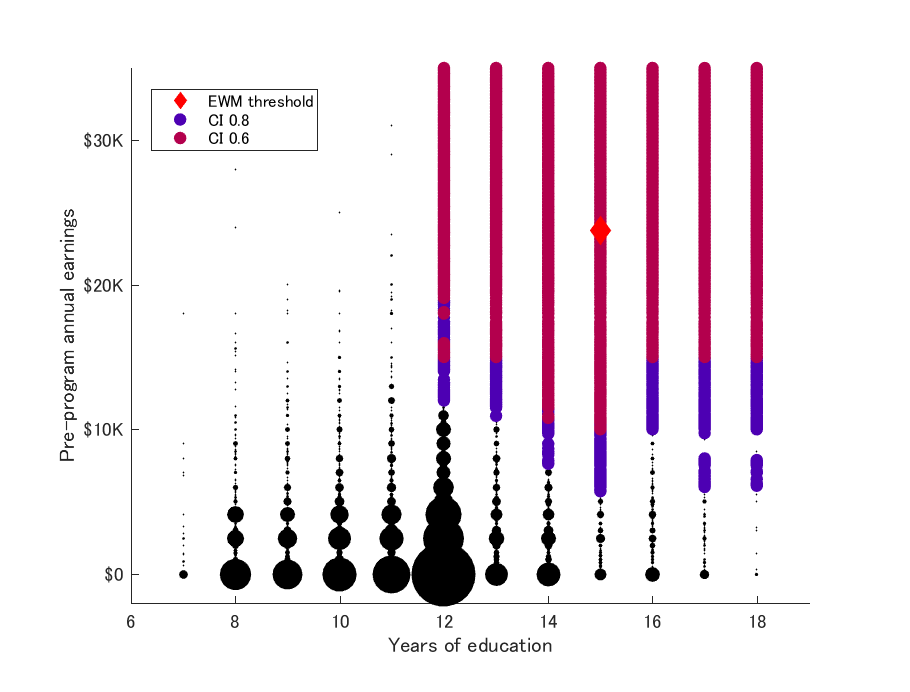
\includegraphics[width=\textwidth]{CIfig_nocost.eps}
  \end{center}
\subcaption*{No treatment cost }
 \end{minipage}
 \begin{minipage}{0.5\hsize}
  \begin{center}
   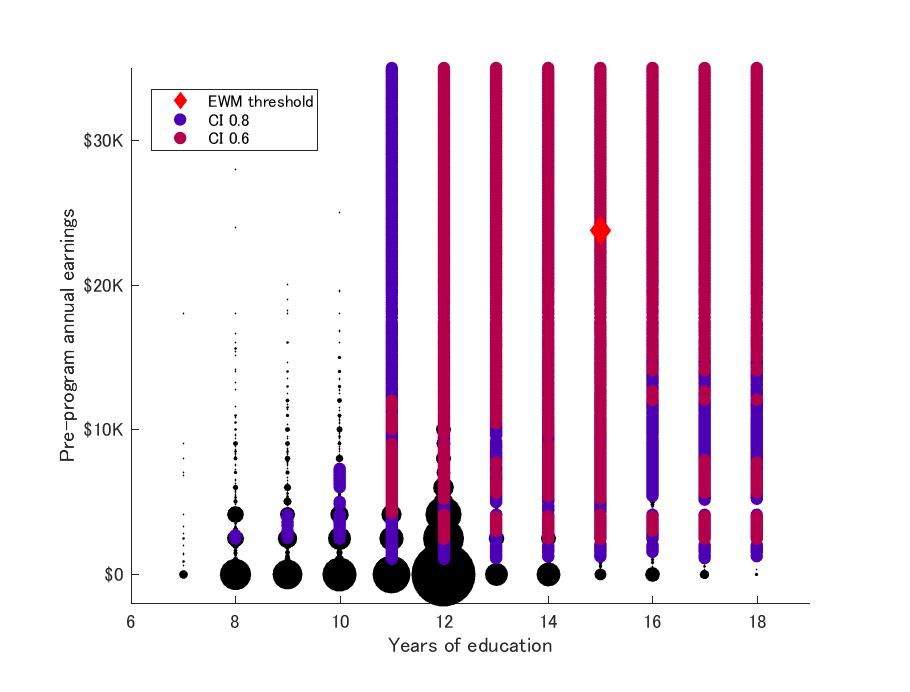
\includegraphics[width=\textwidth]{CIfig_withcost.eps}
  \end{center}
\subcaption*{\$774 cost per assignment}
 \end{minipage}
   \end{tabular}     
\caption{Confidence sets for the optimal policy with confidence levels 0.8 and 0.6 from the threshold class of assignment policies conditioning on years
of education and pre-program earnings}\label{f:nocap}
\end{center}
\end{figure}

%%\begin{figure} 
%%\label{f:nocost}
%%\hspace{5mm}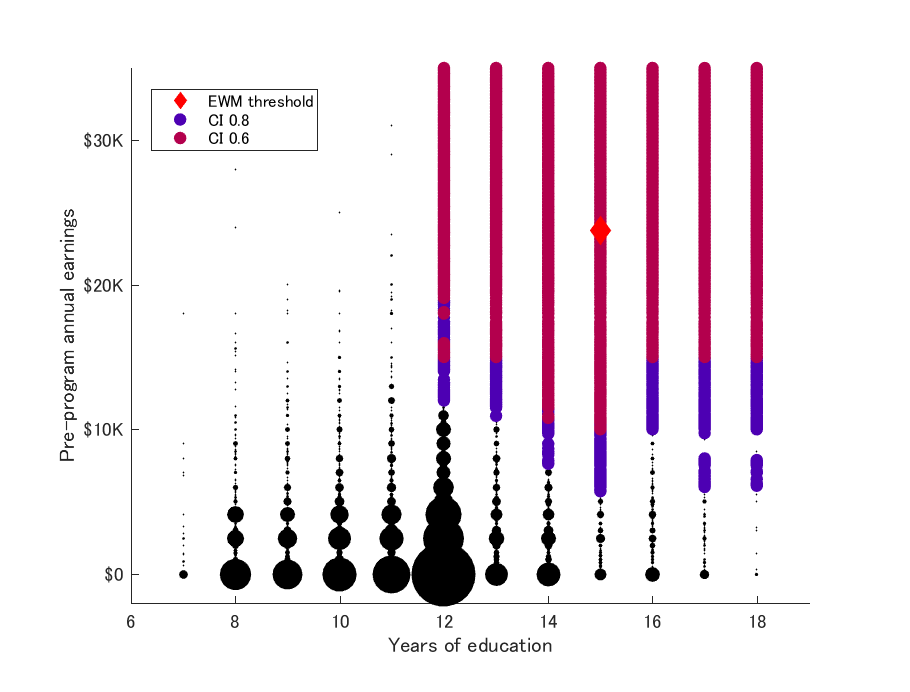
\includegraphics[width=\textwidth]{CIfig_nocost.eps}
%%\caption{Level $0.8$ and $0.6$ confidence set for the optimal policy from the threshold class of assignment policy conditioning on yearsof education and pre-program earnings with no assignment cost}
%%\end{figure}
Figure \ref{f:nocap} illustrates the confidence sets for the optimal threshold policy without capacity constraint. 
The left panel shows the result with no treatment cost and the right panel shows the result with \$744 cost per assignment. 
On the figure, the size of the black dots represents the number of individuals with different covariate value. The red diamond dot is the EWM threshold point that maximizes estimated average outcome proposed in \cite{KT:18}.  The collection of blue dots represents the confidence set of optimal threshold point 
with confidence level $0.8$ and red dots represents the confidence set with level $0.6$. 
In both cases, EWM thresholds are identical (Year of education $\leq$ 15, preprogram earning $\leq$ \$23,776 ) but confidence sets are largely different. 
When the treatment cost is not taken into account, all the threshold assignment policy that sets education threshold below 12 were rejected to be optimal.
For income threshold, all the threshold assignment policy with income thresholds below \$5,700 are rejected with confidence level $0.8$ and below \$10,014 are rejected 
with confidence level $0.6$.\footnote{With confidence level $0.9$, the result for education threshold does not change. The lower bound for income threshold decreases to \$3,083} The result suggests that the data exhibits strong evidence for the lower bound of optimal thresholds points if the treatment were costless.  
The confidence set expands when the treatment cost is imposed. In that case, most of the rules with education threshold below 11 are rejected to be optimal with confidence level $0.8$ and below 12 are rejected with confidence level $0.6$.  
The confidence set contains most of the rules that set the education threshold above 12 and income threshold strictly above \$0 in both confidence level. 

\begin{figure}[t]
\begin{center}
    \begin{tabular}{cc}
 \begin{minipage}{0.5\hsize}
  \begin{center}
   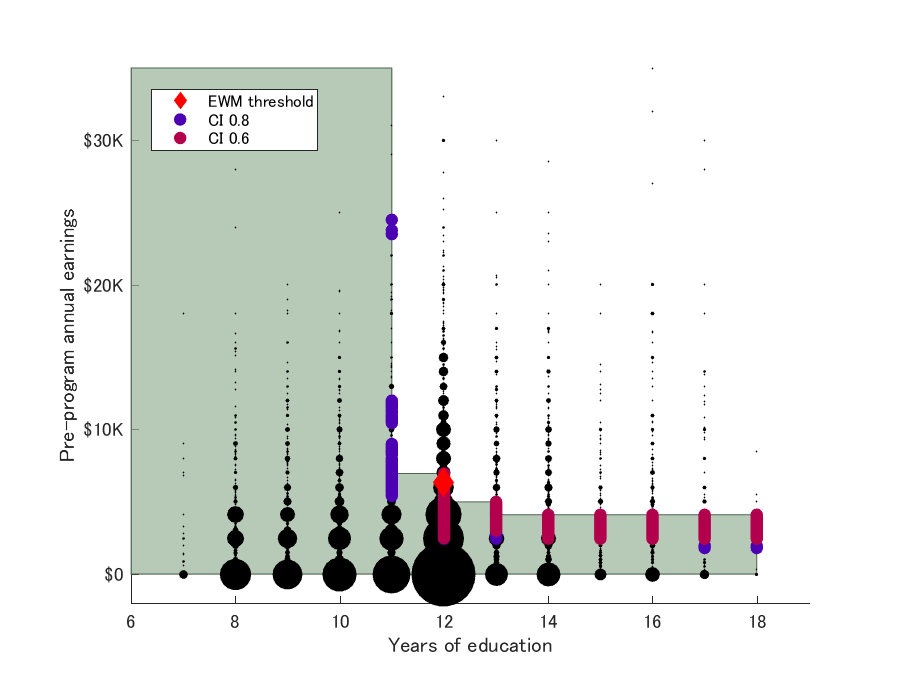
\includegraphics[width=\textwidth]{CIfig_nocost_cap.eps}
  \end{center}
\subcaption*{No treatment cost}
 \end{minipage}
 \begin{minipage}{0.5\hsize}
  \begin{center}
   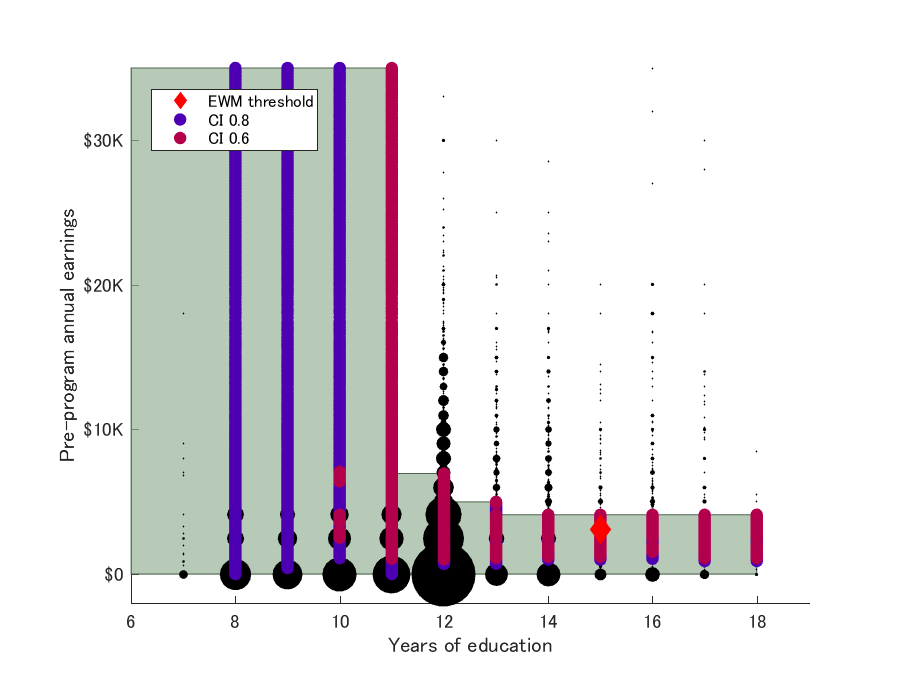
\includegraphics[width=\textwidth]{CIfig_withcost_cap.eps}
  \end{center}
\subcaption*{\$774 cost per assignment}
 \end{minipage}
   \end{tabular}     
\caption{Confidence sets for the optimal policy with confidence levels 0.8 and 0.6 from the threshold class of assignment policies conditioning on years
of education and pre-program earnings with 67\% capacity constraint}\label{f:withcap}
\end{center}
\end{figure}

Figure \ref{f:withcap} illustrates the confidence sets for the optimal threshold policy with capacity constraint. 
The shaded area indicates all the feasible threshold points that assigns individuals to treatment group less than 67\% capacity constraint
The left panel shows the result with no treatment cost and the right panel shows the result with \$744 cost per assignment. 
When treatment costs are not considered, level 0.8 confidence set rejects 
all the threshold assignment policy that sets education threshold below 12 were rejected to be optimal.
When treatment costs are considered, the level $0.8$ confidence set contains all the feasible thresholds points with education threshold above 8 and income threshold strictly above \$0 while the level $0.6$ confidence set rejects most of the policies with education threshold below 10. 


\section{Conclusion}
In this paper, I propose statistical inference methods for treatment assignment policies.  
To obtain the result, I characterize the formal asymptotic property of doubly robust estimator for the average outcome as a function of assignment policies and propose 
asymptotically valid confidence set of the optimal policy and confidence interval for the optimal average outcome. My method is applicable both for
 known propensity score case and for unknown propensity score cases. Simulation results suggest the method works reasonably well in a finite sample. 
I also apply a method to experimental data from the JTPA program and to demonstrate confidence set of optimal assignment policy for a class of threshold assignment policies. 
\newpage
\appendix


\section{Lemmas}
The following list includes notation that will be used in the appendix.
\begin{center}
\begin{tabular}{cl}
\hline 
$a \lesssim b$ & $a\leq Cb$ for some constant $C$ universal in the proof.\\
$N(\mathcal{F},d,\epsilon)$  & For a pseudometric space $(\mathcal{F},d)$, $N(\mathcal{F},d,\epsilon)$ is the minimum number of $\epsilon$-balls\\
 & needed to cover $\mathcal{F}$. \\
$\mathbb{G}_{n}$  & Centered empirical process  $\sqrt{n}(\mathbb{P}_{n}-P)$.\\
$\|\mathbb{G}_{n}\|_{\mathcal{F}}$ & For a collection of functions $\mathcal{F}$, $\|\mathbb{G}_{n}\|_{\mathcal{F}}=\sup_{f\in \mathcal{F}}|\mathbb{G}_{n}(f)|$. \\
$\|f \|_{Q,q}$  & For a measurable function $f$, and a measure $Q$, $\|f \|_{Q,q}=\{\int |f|^{q}dQ\}^{1/q}$.\\
$l^{\infty}(\mathcal{A})$  & The space of bounded functions on $\mathcal{A}$. \\
$C^{\infty}(\mathcal{A})$  & The space of bounded continuous functions on $\mathcal{A}$. \\
$BL_{b}(\mathcal{A})$  & The set of functions on $\mathcal{A}$ with $\sup_{a\in \mathcal{A}} f(a)\leq b$ and $|f(a)-f(a^{\prime})|\leq bd(a,a^{\prime})$. \\
\hline 
\end{tabular}\vspace{2cm}
\end{center}

Before showing the main result, I introduce lemmas and definitions used in the proof of main result. 
\begin{lemma}\label{l:entropy}
Let $\mathcal{F}_{i},\ldots,\mathcal{F}_{k}$ be classes of real valued functions with respective envelope functions $F_{i},\ldots,F_{k}$.  
Let $\phi:\mathbb{R}^{k}\rightarrow \mathbb{R}$ be a map that is Lipschitz in the sense that there exists nonnegative functions $L_{i},\ldots,L_{k}$
such that 
\begin{align*}
|\phi\circ f(x) -\phi\circ g(x)|^{2}\leq \sum_{i=1}^{k}L_{i}(x)^{2}|f_{i}(x)-g_{i}(x)|^{2}
\end{align*}
holds for all $f, g\in \mathcal{F}_{1}\times\cdots \times \mathcal{F}_{k}$ and all $x$. Then, a class of real valued function 
\[\phi\circ (\mathcal{F}_{i},\ldots,\mathcal{F}_{k}) = \{\phi\circ f \ | \ f\in  \mathcal{F}_{1}\times\cdots \times \mathcal{F}_{k}\}\]
has an envelope function $H=|\phi\circ f_{0}|+\sum_{i=1}^{k}L_{i}(F_{i}+|f_{0,i}|)$ where $f_{0}=(f_{0,1},...,f_{0,k})$ is any function satisfying 
\begin{align*}
|\phi\circ f(x) -\phi\circ f_{0}(x)|^{2}\leq \sum_{i=1}^{k}L_{i}(x)^{2}|f_{i}(x)-f_{0,i}(x)|^{2}
\end{align*}
for all $f\in  \mathcal{F}_{1}\times\cdots \times \mathcal{F}_{k}$ and all $x$
$\mathcal{F}_{1}\times\cdots \times \mathcal{F}_{k}$. Moreover, $\phi\circ (\mathcal{F}_{i},\ldots,\mathcal{F}_{k})$ satisfies 
\[\sup_{Q} N(\phi\circ (\mathcal{F}_{i},\ldots,\mathcal{F}_{k}),\|\cdot\|_{Q,2},\|H\|_{Q,2}\epsilon)\leq 
\prod_{i=1}^{k}\sup_{Q_{i}} N(\mathcal{F}_{i},\| \cdot \|_{Q_{i},2},\|F_{i}\|_{Q_{i},2}\epsilon)\]
where the supremum is taken over all finitely discrete probability measures. 
\begin{proof}
For any $f\in \mathcal{F}_{1}\times\cdots \times \mathcal{F}_{k}$, 
\begin{align*}
|\phi\circ f|&\leq |\phi\circ f_{0}| + |\phi\circ f_{0}-\phi\circ f |,\\
&\leq |\phi\circ f_{0}| + \sqrt{\sum_{i=1}^{k}L_{i}^{2}|f_{0,i}-f_{i}|^{2}},\\
&\leq |\phi\circ f_{0}| + \sum_{i=1}^{k}L_{i}(F_{i}+|f_{0,i}|).
\end{align*}
Thus, $H$ is an envelope for $\phi\circ (\mathcal{F}_{i},\ldots,\mathcal{F}_{k})$. Fix $\epsilon>0$ and a finitely discrete probability measures $Q$.
For each $i=1,...,k$ define probability measure $Q^{*}_{i}=\frac{F_{i}^{2}}{\|F_{i}\|_{Q,2}^{2}}Q$.
Take $f, g\in \mathcal{F}_{1}\times\cdots \times \mathcal{F}_{k}$ such that $\|f_{i}-g_{i}\|_{Q^{*}_{i},2}\leq \|F_{i}\|_{Q_{i},2}\epsilon$. Then 
\begin{align*}
|\phi\circ f-\phi\circ g |_{Q,2}&\leq \sqrt{\sum_{i=1}^{k}\|L_{i}|f_{i}-g_{i}|\|_{Q,2}^{2}},\\
&\leq  \epsilon\sqrt{\sum_{i=1}^{k}\|L_{i}\|_{Q}^{2}\|F_{i}\|_{Q^{*}_{i},2}^{2}},\\
&=  \epsilon \sqrt{\sum_{i=1}^{k} \|L_{i}F_{i}\|_{Q,2}^{2}}.\\
\end{align*}
Since $\sum_{i=1}^{k} \|L_{i}F_{i}\|_{Q,2}^{2}\leq \|H\|_{Q,2}^{2}$, the above inequality implies 
\[N(\phi\circ (\mathcal{F}_{i},\ldots,\mathcal{F}_{k}),\|\cdot\|_{Q,2},\|H\|_{Q,2}\epsilon)\leq \prod_{i=1}^{k}N(\mathcal{F}_{i},\| \cdot \|_{Q^{*}_{i},2},\|F_{i}\|_{Q^{*}_{i},2}\epsilon).\]
Taking supremum over $Q$ on both sides shows the result. 
\end{proof}
\end{lemma}
I will use the following Corollary to the above lemma.  
\begin{corollary}\label{c:entropy}
Let $\mathcal{F}_{1}$ and $\mathcal{F}_{2}$ be classes of real valued functions with envelope functions $F_{1}$ and $F_{2}$ respectively.
\begin{itemize}
\item[{(i)}]  The class of functions 
\[\mathcal{F}_{1}\cdot\mathcal{F}_{2}=\{fg\ | \ f\in \mathcal{F}_{1}, g\in \mathcal{F}_{2}\} \]
has an envelope function $H=2\sqrt{2}FG$ and satisfies
\[\sup_{Q}N(\mathcal{F}_{1}\cdot\mathcal{F}_{2},\|\cdot\|_{Q,2},\|H\|_{Q,2}\epsilon)\leq 
\sup_{Q}N(\mathcal{F}_{1},\|\cdot\|_{Q,2},\|F_{1}\|_{Q,2}\epsilon)\sup_{Q}N(\mathcal{F}_{2},\|\cdot\|_{Q,2},\|F_{2}\|_{Q,2}\epsilon)\]
where $Q$ is taken over all finitely discrete probability measures.
\item[{(ii)}] For any measurable functions $g$ and $h$,
 the class of function 
 \[\mathcal{F}_{1}g+h=\{fg+h\ | \ f\in \mathcal{F}\} \]
has an envelope $H=F_{1}|g|+|h|$ and satisfies
\[\sup_{Q}N(\mathcal{F}_{1}g+h,\|\cdot\|_{Q,2},\|H\|_{Q,2}\epsilon)\leq 
\sup_{Q}N(\mathcal{F}_{1},\|\cdot\|_{Q,2},\|F_{1}\|_{Q,2}\epsilon)\]
where $Q$ is taken over all finitely discrete probability measures.
\item[{(iii)}] If $\inf_{f\in \mathcal{F}_{1}}\inf_{x}|f(x)|>c$ for some constant $c>0$.
 Then the class of functions  
\[\mathcal{F}_{1}^{-1}=\{f^{-1}\ | \ f\in \mathcal{F}_{1}\}\]
has an envelope function $H=2/c+F_{1}/c^{2}$ and satisfies 
\[\sup_{Q}N(\mathcal{F}_{1}^{-1},\|\cdot\|_{Q,2},\|H\|_{Q,2}\epsilon)\leq 
\sup_{Q}N(\mathcal{F}_{1},\|\cdot\|_{Q,2},\|F_{1}\|_{Q,2}\epsilon)\]
where $Q$  is taken over all finitely discrete probability measures.
\end{itemize}
\end{corollary}

\textbf{Proof of (i).} 
Let $\phi\circ f=f_{1}+f_{2}$ for $(f_{1},f_{2})\in \mathcal{F}_{1}\times \mathcal{F}_{2}$. 
Then I can apply lemma \ref{l:entropy} with $L_{1}=L_{2}=1$ and $f_{0}=0$. 

\textbf{Proof of (ii).} 
Let $\phi\circ f=f_{1}f_{2}$ for $(f_{1},f_{2})\in \mathcal{F}_{1}\times \mathcal{F}_{2}$. Since  
\begin{align*}
|\phi\circ f(x)-\phi\circ g(x)|^{2}&\leq \{F_{2}|f_{1}(x)-g_{1}(x)|+F_{1}|f_{2}(x)-g_{2}(x)|\}^{2}\\ 
&\leq 2\{F_{2}\}^{2}|f_{1}(x)-g_{1}(x)|^{2}+2\{F_{1}\}^{2}|f_{2}(x)-g_{2}(x)|^{2}
\end{align*}
holds for any $f, g$ in $\mathcal{F}_{1}\times \mathcal{F}_{2}$, I can apply 
lemma \ref{l:entropy} with $L_{1}=\sqrt{2}F_{2}$, $L_{2}=\sqrt{2}F_{1}$ and $f_{0}=0$. 

\textbf{Proof of (iii).} 
Let $k=1$ and $\phi\circ f= fg+h$ for $f\in \mathcal{F}_{1}$. Then, the result follows from 
lemma \ref{l:entropy} with $L_{1}=|g|$ and $f_{0}=0$.  

\textbf{Proof of (iv).} 
Let $k=1$ and $\phi\circ f= f^{-1}$ for $f\in \mathcal{F}_{1}$.
Since 
\[|f(x)^{-1}-g(x)^{-1}|^{2}\leq \frac{1}{c^{2}}|f(x)-g(x)|^{2}\]
for any $f, g$ in $\mathcal{F}_{1}$ and any $x$, 
the result follows from lemma \ref{l:entropy} with $L_{1}=|c^{-2}|$ and $f_{0}=c$.  


The following maximal inequality and deviation inequality is due to Theorem 5.1 and Corollary 5.1 in \cite{CCK:14}. 
\begin{lemma}\label{l:deviation}
Let $\mathcal{F}$ be a class of pointwise measurable function with a measurable envelope $F$ satisfying $E[F^{q}]<\infty$ for $q\geq 2$. 
Let $M=\max_{i=1,...,n}F(X_{i})$ and $\sup_{f\in \mathcal{F}}E[f^{2}]\leq \sigma^{2}\leq \|F\|_{P,2}^{2}$. 
Then, for any $\alpha>0$ and any $t\geq 1$,
 the centered empirical process $\mathbb{G}_{n}=\frac{1}{\sqrt{n}}\sum_{i=1}^{n}\{f(X_{i})-Pf\}$ satisfies deviation inequality 
\begin{align*}
\|\mathbb{G}_{n}\|_{\mathcal{F}}\leq (1+\alpha)E[\|\mathbb{G}_{n}\|_{\mathcal{F}}]+K(q)\left[(\sqrt{t}\sigma+\frac{\sqrt{t}\|M\|_{P,q}}{n^{1/2}})+
\frac{t\|M\|_{P,2}}{\alpha n^{1/2}}\right]
\end{align*}
 with probability at least $1-t^{-q/2}$ where $K(q)$ is a constant depends only on $q$.
 If 
\[\sup_{Q}N(\mathcal{F},\|\cdot\|_{Q,2},\|F\|_{Q,2}\epsilon)\leq (a/\epsilon)^{v}\]
for some $a\geq e$ and $v\geq 1$, it also satisfies the maximal inequality
\[E[\|\mathbb{G}_{n}\|_{\mathcal{F}}]\lesssim  \sqrt{\sigma^{2} v\ln\left(\frac{ a\|F\|_{P,2}}{\sigma}\right)}+\frac{\|M\|_{P,2}}{n^{1/2}}v\ln\left(\frac{ a\|F\|_{P,2}}{\sigma}\right).\]
Combining these two inequalities and taking $t=\ln (n)$ and $a\geq \max\{n,e\}$ shows 
\[\|\mathbb{G}_{n}\|_{\mathcal{F}}\leq K(q)\left\{\sqrt{\sigma^{2} v\ln\left(\frac{ a\|F\|_{P,2}}{\sigma}\right)}+\frac{\|M\|_{P,q}}{n^{1/2}}v\ln\left(\frac{ a\|F\|_{P,2}}{\sigma}\right)\right\}\]
with probability at least $1-\ln(n)^{-1}$ where $K(q)$ is a constant depends only on $q$. 
\end{lemma}


\begin{lemma}\label{l:residual}
Suppose assumption G, D, N and B hold.
Let $\mathcal{G}$ be a collection of feasible policies and $\mathcal{M}^{*}_{1,n}$, $\mathcal{E}^{*}_{n}$ be the sets in assumption N (ib) and (iib). 
Define $\mathcal{F}_{1,n}$, $\mathcal{F}_{2,n}$ and $\mathcal{F}_{3,n}$ 
\begin{align*}
\mathcal{F}_{1,n}&=\left\{\left\{1-\frac{d}{e(x)}\right\}\{m_{1}^{*}(x)-m_{1}(x)\}1\{x\in G\}\ | \ m_{1}^{*}\in \mathcal{M}^{*}_{1,n}, G\in \mathcal{G}\right\}\\
\mathcal{F}_{2,n}&=\left\{\{y-m_{1}(x)\}d\left\{\frac{1}{e^{*}(x)}-\frac{1}{e(X)}\right\}1\{x\in G\} \ |\ e^{*}\in \mathcal{E}^{*}_{n},G\in \mathcal{G}\right\}\\
\mathcal{F}_{3,n}&=\left\{\{m_{1}^{*}(x)-m_{1}(x)\}d\left\{\frac{1}{e^{*}(x)}-\frac{1}{e(X)}\right\}1\{x\in G\} \ | \ m_{1}^{*}\in \mathcal{M}^{*}_{1,n}, 
e^{*}\in \mathcal{E}^{*}_{n},G\in \mathcal{G}\right\}.
\end{align*}
Similarly, define $\mathcal{F}^{B}_{j,n}$ 
\begin{align*}
\mathcal{F}_{j,n}^{B}&=\{ fB\ | \ f\in \mathcal{F}_{j,n}\}
\end{align*}
for $j= 1,2,3$ where $B$ is a bootstrap weight.  Then for $j=1,2,3,$
\begin{align*}
\|\mathbb{G}_{n}\|_{\mathcal{F}_{j,n}}<o(1), \qquad \|\mathbb{G}_{n}\|_{\mathcal{F}_{j,n}^{B}}<o(1)  
\end{align*}
hold with probability at least $1-\ln n^{-1}$. 
\begin{proof}
By assumption G, $\mathcal{G}$ is a VC class of sets. Thus, by theorem 2.6.4 in \cite{VW:96}, 
\[\sup_{Q}\ln N(\{1\{X\in G\}\}_{G\in \mathcal{G}},\|\cdot\|_{Q,2},C_{1}\epsilon)\lesssim  v\ln(e/\epsilon)\]
for some fixed constant $v$ where the supremum is taken over all finitely discrete probability measures.
Since $v$ is fixed, I may assume $v\leq \min\{v_{m},v_{e}\}$. 

In the following, I will apply lemma \ref{l:deviation} to $\mathcal{F}_{j,n}$. 
First, I show the metric entropy bound conditions. 
By assumption D, $e(X)\in (\eta,1-\eta)$. Moreover, $E[|Y|^{q}]$ and $m_{d}$ is bounded uniformly over $P$. 
By assumption N,  $e^{*}(x)\in \mathcal{E}^{*}_{n}$ satisfies $e^{*}(x)\in (\eta/2,1-\eta/2)$ and $m^{*}_{d}\in \mathcal{M}^{*}_{d,n}$ is bounded.
Thus, applying corollary \ref{c:entropy} (i) and (ii) to $\mathcal{M}^{*}_{1,n}$ and $\{1\{X\in G\}\}_{G\in \mathcal{G}}$ shows 
\[\sup_{Q}\ln N(\mathcal{F}_{1,n},\|\cdot\|_{Q,2},C_{1}\epsilon)\lesssim  v_{m}\ln(a/\epsilon)+v\ln(e/\epsilon)< 2v_{m}\ln(a/\epsilon)\]
with some constant envelope $C_{1}$. Applying corollary \ref{c:entropy} (ii) and (iii) to $\mathcal{E}^{*}_{n}$ and $\{1\{X\in G\}\}_{G\in \mathcal{G}}$ shows 
\[\sup_{Q}\ln N(\mathcal{F}_{2,n},\|\cdot \|_{Q,2},\|F_{2}\|_{Q,2}\epsilon)\lesssim v_{e}\ln(a/\epsilon)+v\ln(e/\epsilon)< 2v_{e}\ln(a/\epsilon).\]
with a measurable envelope $F_{2}$ with bounded $q$-th moment $E_{P}[|F|^{q}]$ uniformly over $P$. Similarly, applying corollary \ref{c:entropy} (i), (ii) and (iii) 
to $\mathcal{M}^{*}_{1,n}$, $\mathcal{E}^{*}_{n}$ and $\{1\{X\in G\}\}_{G\in \mathcal{G}}$ shows
\[\sup_{Q}\ln N(\mathcal{F}_{3,n},\|\cdot\|_{Q,2},C_{3}\epsilon )\lesssim v_{m}\ln(a/\epsilon)+v_{e}\ln(a/\epsilon)+v\ln(e/\epsilon)< 3\max\{v_{m},v_{e}\}\ln(a/\epsilon).\]

Second, I derive the bounds for $\sup_{f\in \mathcal{F}_{j,n}}E_{P}[f^{2}]$. 
For $f\in \mathcal{F}_{1,n}$, 
\begin{align*}
E_{P}[f^{2}]&=E_{P}\left[\left\{1-\frac{D}{e(X)}\right\}^{2}\left\{m^{*}_{1}(X)-m_{1}(X)\right\}^{2}1\{X\in G\}^{2}\right]\\
&\lesssim E_{P}[\left\{m^{*}_{1}(X_{i})-m_{1}(X_{i})\right\}^{2}]\\
&\leq \delta_{m}^{2}
\end{align*}
holds. For $f\in \mathcal{F}_{2,n}$, 
\begin{align*}
E_{P}[f^{2}]&=E_{P}\left[\left\{\{Y-m_{1}(X)\}D\left\{\frac{1}{e^{*}(X)}-\frac{1}{e(X)}\right\}1\{X\in G\}\right\}^{2}\right]\\
&\leq E_{P}\left[\left. E_{P}\left[\left\{ \frac{\{Y-m_{1}(X)\}D}{e^{*}(X)e(X)}\right\}^{2}\right| X \right]\left\{e^{*}(X)-e(X)\right\}^{2}\right]\\
&\lesssim \delta_{e}^{2}
\end{align*}
holds sine $E_{P}[Y(d)^{2}|X]<\infty$ uniformly over $P$ and $\{e(X)e^{*}(x)\}^{-1}\geq \eta^{2}/4$.
For $f\in \mathcal{F}_{3,n}$,
\begin{align*}
\sup_{f\in \mathcal{F}_{3,n}}E_{P}[f^{2}] &=E_{P}\left[\left\{D\{m_{1}^{*}(X)-m_{1}(X)\}\frac{\left\{e^{*}(X)-e(X)\right\}}{e^{*}(X)e(X)}\right\}^{2}1\{X\in G\}^{2}\right]\\
&\lesssim E_{P}[\{m_{1}^{*}(X_{i})-m_{1}(X_{i})\}^{2}\{e^{*}(X_{i})-e(X_{i})\}^{2}]\\
&\leq \max\{C_{m}^{2},\eta^{2}/4\}\min\{\delta_{m},\delta_{e}\}
\end{align*}
holds since $|m_{1}^{*}(x)-m_{1}(x)|<C_{m}$ and $|e(X)-e^{*}(x)|< \eta/2$. 
Thus, I obtain 
\begin{align*}
\sup_{f\in \mathcal{F}_{1,n}}E_{P}[f^{2}]\lesssim \delta_{m}^{2},\ \sup_{f\in \mathcal{F}_{2,n}}E_{P}[f^{2}]\lesssim \delta_{e}^{2},\ \sup_{f\in \mathcal{F}_{3,n}}E_{P}[f^{2}]\lesssim \min\{\delta_{e},\delta_{m}\}^{2}
\end{align*}
uniformly over $P$. Finally, note that 
\[E_{P}[\{\max_{i=1,\ldots,n}|F_{2,i}|\}^{2}]\leq E_{P}[\{\max_{i=1,\ldots,n}|F_{2,i}|\}^{q}]^{2/q}\leq n^{2/q}E_{P}[|F_{2}|^{q}]\]
where $F_{2,i}=F_{2}(Y_{i},D_{i},X_{i})$.
Thus, by lemma \ref{l:deviation}, deviation inequalities 
\begin{align*}
\|\mathbb{G}_{n}\|_{\mathcal{F}_{1,n}}&\lesssim
 \sqrt{ \delta_{m}^{2} v_{m}\ln\left(\frac{a}{ \delta_{m}}\right)}+\frac{v_{m}}{n^{1/2}}\ln\left(\frac{a}{ \delta_{m}}\right), \\ 
\|\mathbb{G}_{n}\|_{\mathcal{F}_{2,n}}&\lesssim
 \sqrt{ \delta_{m}^{2} v_{e}\ln\left(\frac{a}{ \delta_{e}}\right)}+\frac{v_{e}}{n^{(q-2)/2q}}\ln\left(\frac{a}{ \delta_{e}}\right),\\
 \|\mathbb{G}_{n}\|_{\mathcal{F}_{3,n}}&\lesssim
 \sqrt{ \delta_{m}^{2} \bar{v}\ln\left(\frac{a}{\underline{\delta}}\right)}+\frac{\bar{v}}{n^{1/2}}\ln\left(\frac{a}{\underline{\delta}}\right), 
\end{align*}
hold with probability at least $1-\ln(n)^{-1}$. By assumption N, this implies $\|\mathbb{G}_{n}\|_{\mathcal{F}_{1,n}}< o(1)$ for $j= 1,2,3$.

By applying corollary \ref{c:entropy} (ii) to $\mathcal{F}_{j,n}$ and $B$, I obtain
\begin{align*}
\sup_{Q}\ln N(\mathcal{F}_{1,n}^{B},\|\cdot\|_{Q,2},C_{1}\|B\|_{Q,2}\epsilon)&\lesssim  v_{m}\ln(a/\epsilon),\\
\sup_{Q}\ln N(\mathcal{F}_{2,n}^{B},\|\cdot \|_{Q,2},\|F_{2}|B|\|_{Q,2}\epsilon)&\lesssim v_{e}\ln(a/\epsilon),\\
\sup_{Q}\ln N(\mathcal{F}_{3,n}^{B},\|\cdot\|_{Q,2},C_{3}\|B\|_{Q,2}\epsilon )&\lesssim \max\{v_{m},v_{e}\}\ln(a/\epsilon).
\end{align*}
Since $B$ is independent from the data and $E_{B}[B^{2}]=1$, 
\[\sup_{f\in\mathcal{F}_{j,n}^{B}}E_{P}[\{fB\}^{2}]=\sup_{f\in\mathcal{F}_{j,n}}E_{P}[f^{2}]\]
for $j=1,2,3$.
Moreover, since $B$ is Sub-Gaussian, $E_{B}[\exp(aB^{2})]$ is bounded for some $a>0$. Thus, 
\begin{align*}
\exp(aE_{B}[\{\max_{i=1,\ldots,n}|B_{i}|\}^{2}])
&=\exp(aE_{B}[\max_{i=1,\ldots,n}B_{i}^{2}])\\
&\leq E_{B}\exp(a\max_{i=1,\ldots,n}B_{i}^{2})\\
&\leq nE_{B}[\exp(aB^{2})]. 
\end{align*}
Taking $\ln(\cdot)$ on both sides shows 
 $E_{B}[\{\max_{i=1,...,n}|B_{i}|\}^{2}]\lesssim \ln(n)$. This implies   
\begin{align*}
E_{P}[\{\max_{i=1,...,n}C_{1}|B_{i}|\}^{2}]&\lesssim C_{1}^{2}\ln(n)\\
E_{P}[\{\max_{i=1,...,n}F_{2,i}|B_{i}|\}^{2}]&\lesssim n^{2/q}E_{P}[|F_{2}|^{q}]\ln(n)\\
E_{P}[\{\max_{i=1,...,n}C_{3}|B_{i}|\}^{2}]&\lesssim C_{3}^{2}\ln(n),
\end{align*}
where $F_{2,i}=F_{2}(Y_{i},D_{i},X_{i})$. 
By applying lemma \ref{l:deviation}, deviation inequalities 
\begin{align*}
\|\mathbb{G}_{n}\|_{\mathcal{F}_{1,n}^{B}}&\lesssim 
\sqrt{ \delta_{m}^{2} v_{m}\ln\left(\frac{a}{ \delta_{m}}\right)}+\frac{\ln(n)v_{m}}{n^{1/2}}\ln\left(\frac{a}{ \delta_{m}}\right),\\
\|\mathbb{G}_{n}\|_{\mathcal{F}_{2,n}^{B}}&\lesssim  \sqrt{ \delta_{m}^{2} v_{e}\ln\left(\frac{a}{ \delta_{e}}\right)}+\frac{\ln(n)v_{e}}{n^{(q-2)/2q}}\ln\left(\frac{a}{ \delta_{e}}\right),\\ 
\|\mathbb{G}_{n}\|_{\mathcal{F}_{3,n}^{B}}&\lesssim 
\sqrt{ \delta_{m}^{2} \bar{v}\ln\left(\frac{a}{\underline{\delta}}\right)}+\frac{\ln(n)\bar{v}}{n^{1/2}}\ln\left(\frac{a}{ \underline{\delta}}\right),\\
\end{align*}
hold with probability at least $1-\ln(n)^{-1}$. The result follows from assumption N.  
\end{proof}
\end{lemma}

I define the pseudometric $d_{g}$ on $\mathcal{G}$ as follows. 
\begin{defP}
Suppose assumption D holds. Let $\mu_{X}=\times_{k=1}^{d_{x}}\mu_{X_{k}}$ defined in assumption D (v).  
Let $\mathcal{G}$ be a fixed collection of feasible assignment policies satisfying assumption G. 
Suppose $\mathcal{G}$ depends on a subset of characteristics $\tilde{X}=(\tilde{X}_{1},\ldots,\tilde{X}_{J})$ with $J\leq d_{x}$. 
Define pseudometric $d_{g}(\cdot,\cdot)$ on $\mathcal{G}$ as 
\[\int |1\{\tilde{X}\in G\}-1\{\tilde{X}\in G^{\prime}\}| d\mu_{\tilde{X}},\]
where $\mu_{\tilde{X}}=\times_{k=1}^{J}\mu_{\tilde{X}_{k}}$. 
\end{defP} 
Following lemma presents properties of $d_{g}$ that will be used in the proof of Theorems. 
\begin{lemma}\label{l:metric}
Suppose assumption D and G holds. Then the following properties hold. 
\begin{itemize}
\item[{(i)}] $\sup_{G,G^{\prime}\in \mathcal{G}}d_{g}(G,G^{\prime})<\infty$

\item[{(ii)}] $(\mathcal{G},d_{g})$ is totally bounded. Moreover, the covering number satisfies 
\[N(\mathcal{G},d_{g},\epsilon)<C(e/\epsilon)^{v}\]
for some universal constant $C$ and $v$.

\item[{(iii)}] There exists a universal constant $C$ such that $P(G\Delta G^{\prime}) \leq Cd_{g}(G, G^{\prime})$ for any $G,G^{\prime}\in \mathcal{G}$ 
holds uniformly over $P$ satisfying assumption D.

\item[{(iv)}] $W(G)$ is continuous with respect to $d_{g}$.

\end{itemize}
\end{lemma}
\textbf{Proof of (i).}
By assumption N, $\max_{k=1,\ldots,d_{x}}|X_{k}|<C_{X}$ and $\prod_{k=1}^{J}\mu_{\tilde{X}_{k}}((-C_{X},C_{X}))<\infty$.
 Thus,   
\[\sup_{G,G^{\prime}\in \mathcal{G}}d_{G}(G,G^{\prime})\leq \prod_{k=1}^{J}\mu_{\tilde{X}_{k}}((-C_{X},C_{X}))<\infty.\]

\textbf{Proof of (ii).}
By assumption G, $\mathcal{G}$ is a VC class. Thus, for any probability measure $Q$ on $\mathbb{R}^{J}$, 
\[N(\{1\{\tilde{X}\in G\}\}_{G\in \mathcal{G}},\|\cdot\|_{Q,1},\epsilon)\lesssim (1/\epsilon)^{v}<\infty\]
holds for some fixed constant $v$. 
Since $\mu_{\tilde{X}}$ is bounded on $\times^{J}(-C_{X},C_{X})\subset \mathbb{R}^{J}$,  
\[\tilde{Q}=\frac{1\{X\in (-C_{X},C_{X})^{J}\}}{\prod_{k=1}^{J}\mu_{\tilde{X}_{k}}((-C_{X},C_{X}))}\mu_{\tilde{X}}\]
is a probability measure on $\mathbb{R}^{J}$, where $\times^{J}$ is a cartesian product. 
Since $G\subset \times^{J}(-C_{X},C_{X})$ for any $G\in \mathcal{G}$, 
\begin{align*}
N\left(\{1\{\tilde{X}\in G\}\}_{G\in \mathcal{G}},\|\cdot\|_{\mu_{\tilde{X}},1},\prod_{k=1}^{J}\mu_{\tilde{X}_{k}}((-C_{X},C_{X}))\epsilon\right)
&=N(\{1\{\tilde{X}\in G\}\}_{G\in \mathcal{G}},\|\cdot\|_{\tilde{Q},1},\epsilon)\\
&\lesssim (1/\epsilon)^{v}.
\end{align*}
By definition $d_{g}(G,G^{\prime})=\|1\{X\in G\}-1\{X\in G^{\prime}\} \|_{\mu_{\tilde{X}},1}$. 
Thus, 
\[N(\mathcal{G},d_{g},\epsilon)\lesssim (1/\epsilon)^{v}<\infty.\]

\textbf{Proof of (iii).} By assumption D (v), $\tilde{X}$ has a density $f_{\tilde{X}}<C_{x}$ with respect to $\mu_{\tilde{X}}=\times_{k=1}^{J}\mu_{\tilde{X}_{k}}$. 
Thus, 
\begin{align*}
P(G\Delta G^{\prime})&=\int |1\{X\in G\}-1\{X\in G^{\prime}\}|dP_{X}\\
&=\int |1\{\tilde{X}\in G\}-1\{\tilde{X}\in G^{\prime}\}|dP_{\tilde{X}}\\
&= \int |1\{X\in G\}-1\{X\in G^{\prime}\}|f_{\tilde{X}} d\mu_{\tilde{X}}\\
&\leq C_{f}d_{g}(G,G^{\prime}).
\end{align*}

\textbf{Proof of (iv).} Since $m_{d}$ is bounded by assumption D, 
\begin{align*}
|W(G)-W(G^{\prime})|&=\left|E_{P}[ m_{1}(X)-m_{0}(X)1\{X\in G\}-1\{X\not\in G^{\prime}\}]\right|,\\
&\leq E_{P}[\left| m_{1}(X)-m_{0}(X)\right|\left|1\{X\in G\}-1\{X\not\in G^{\prime}\}\right|],\\
&\lesssim d_{g}(G,G^{\prime}).
\end{align*}


\section{Proof of main results}
\subsection*{\bf{Proof of Theorem 1}}
Let $P_{n}$ be a sequence of data generating processes satisfying the assumptions in theorem. 
Note that 
\begin{align*}
&\sqrt{n}\{\hat{W}(G)-W(G)\}=\frac{1}{\sqrt{n}}\sum_{i=1}^{n}s_{G}(Y_{i},D_{i},X_{i})\\
&+\frac{1}{\sqrt{n}}\sum_{i=1}^{n}\left(\frac{\{Y_{i}-\hat{m}_{1}(X_{i})\}D_{i}}{\hat{e}(X_{i})}-\frac{\{Y_{i}-m_{1}(X_{i})\}D_{i}}{e(X_{i})}+\hat{m}_{1}(X_{i})
-m_{1}(X_{i})\right)1\{X\in G\}\\
&+
\frac{1}{\sqrt{n}}\sum_{i=1}^{n}\left(\frac{\{Y_{i}-\hat{m}_{0}(X_{i})\}(1-D_{i})}{1-\hat{e}(X_{i})}-\frac{\{Y_{i}-m_{0}(X_{i})\}(1-D_{i})}{1-e(X_{i})}+\hat{m}_{0}(X_{i})
-m_{0}(X_{i})\right)1\{X\not\in G\}\\
&=\frac{1}{\sqrt{n}}\sum_{i=1}^{n}s_{G}(Y_{i},D_{i},X_{i})+R+R^{c}.
\end{align*}
Thus, the result follows if 
\begin{align}
\sup_{h\in BL_{1}(l^{\infty}(\mathcal{G}))}\left|E_{P_{n}}\left[h\left(\frac{1}{\sqrt{n}}\sum_{i=1}^{n}s_{G}(Y_{i},D_{i},X_{i})\right)\right]-E[h(Z_{P_{n}})]\right|\rightarrow 0,\label{eq:asylin}\\
\sup_{G\in \mathcal{G}}|R|=o_{P_{n}}(1),\qquad \sup_{G\in \mathcal{G}}|R^{c}|=o_{P_{n}}(1).\label{eq:r1}
\end{align}
I first show (\ref{eq:r1}). 
Since the proof for $\sup_{G\in \mathcal{G}}|R|=o_{P_{n}}(1)$ and $\sup_{G\in \mathcal{G}}|R^{c}|=o_{P_{n}}(1)$
 are identical, I only present the proof for $\sup_{G\in \mathcal{G}}|R|=o_{P_{n}}(1)$. 
Note that $R$ is decomposed as 
\begin{align*}
R=R_{1}+R_{2}+R_{3}
\end{align*}
where 
\begin{align*}
R_{1}&= \frac{1}{\sqrt{n}}\sum_{i=1}^{n}\left\{1-\frac{D_{i}}{e(X_{i})}\right\}\{\hat{m}_{1}(x_{i})-m_{1}(X_{i})\}1\{X_{i}\in G\},\\
R_{2}&=\frac{1}{\sqrt{n}}\sum_{i=1}^{n}D_{i}\{Y_{i}-m_{1}(X_{i})\}\left\{\frac{1}{\hat{e}(X_{i})}-\frac{1}{e(X_{i})}\right\}1\{X_{i}\in G\},\\
R_{3}&=\frac{1}{\sqrt{n}}\sum_{i=1}^{n}D_{i}\{\hat{m}_{1}(X_{i})-m_{1}(X_{i})\}\left\{\frac{1}{\hat{e}(X_{i})}-\frac{1}{e(X_{i})}\right\}1\{X_{i}\in G\}.
\end{align*}
Let $\mathcal{F}_{1,n}$, $\mathcal{F}_{2,n}$ and $\mathcal{F}_{3,n}$ be collections of functions defined in lemma \ref{l:residual}. 

By assumption N, $\hat{m}_{1}\in \mathcal{M}^{*}_{1,n}$ holds with probability at least $1-\Delta_{n}$. Thus, 
\begin{align*}
\sup_{G\in \mathcal{G}}R_{1}&\leq 
\sup_{(m_{1}^{*},G)\in  \mathcal{M}^{*}_{1,n}\times \mathcal{G}}\left|\left\{1-\frac{D_{i}}{e(X_{i})}\right\}\left\{m^{*}_{1}(X_{i})-m_{1}(X_{i})\right\}1\{X_{i}\in G\}\right|\\
&=\sup_{f\in \mathcal{F}_{1,n}}\left|\frac{1}{\sqrt{n}}\sum_{i=1}^{n}f\right|
\end{align*}
also holds with probability with probability at least $1-\Delta_{n}$. 
By law of iterated expectation,
\begin{align*}
E_{P_{n}}[f]&=E_{P_{n}}\left[\left\{1-\frac{D}{e(X)}\right\}\{m_{1}^{*}(X)-m_{1}(X)\}1\{X\in G\}\right]\\
&=E_{P_{n}}\left[\left\{1-\frac{E\left[D|X\right]}{e(X)} \right\}\{m_{1}^{*}(X)-m_{1}(X)\}1\{X\in G\}\right]\\
&=0
\end{align*}
holds for any $f\in \mathcal{F}_{1,n}$.  
Thus, 
\[\sup_{f\in \mathcal{F}_{1,n}}\left|\frac{1}{\sqrt{n}}\sum_{i=1}^{n}f\right|=\|\mathbb{G}_{n}\|_{\mathcal{F}_{1,n}}.\]
By lemma \ref{l:residual}, $\|\mathbb{G}_{n}\|_{\mathcal{F}_{1,n}}\lesssim o(1)$
holds with probability at least $1-\ln(n)^{-1}$. Thus, 
$\sup_{G\in \mathcal{G}}R_{1}<o(1)$ holds with probability at least $1-\Delta_{n}-\ln(n)^{-1}$. 


By Assumption N, 
$\hat{e}\in \mathcal{E}^{*}_{n}$
with probability at least $1-\Delta_{n}$. Thus,  
\begin{align*}
\sup_{G\in\mathcal{G}}|R_{2}| &\leq \sup_{(e^{*},W)\in \mathcal{E}^{*}_{n}\times \mathcal{G}}\left|\frac{1}{\sqrt{n}}\sum_{i=1}^{n}\{Y_{i}-m_{1}(X_{i})\}D_{i}\left\{\frac{1}{e^{*}(X_{i})}-\frac{1}{e(X_{i})}\right\}1\{X_{i}\in G\}\right|\\
&=\sup_{f\in\mathcal{F}_{2,n}}\left|\frac{1}{\sqrt{n}}\sum_{i=1}^{n}f\right|
\end{align*}
holds with probability at least $1-\Delta_{n}$. By law of iterated expectation,  
\begin{align*}
E_{P_{n}}[f]&=E\left[\{Y-m_{1}(X)\}D\left\{\frac{1}{e^{*}(X)}-\frac{1}{e(X)}\right\}1\{X\in G\}\right]\\
&=E_{P_{n}}\left[\{E[Y|X,D=1]-m_{1}(X)\}D\left\{\frac{1}{e^{*}(X)}-\frac{1}{e(X)}\right\}1\{X\in G\}\right]\\
&=0
\end{align*}
holds for any $f\in \mathcal{F}_{2,n}$. Thus, 
\[\left\|\frac{1}{\sqrt{n}}\sum_{i=1}^{n}f\right\|_{\mathcal{F}_{2,n}}=\|\mathbb{G}_{n}\|_{\mathcal{F}_{2,n}}.\]
By lemma \ref{l:residual}, 
$\|\mathbb{G}_{n}\|_{\mathcal{F}_{2,n}\cdot \mathcal{G}}\lesssim o(1)$
holds with probability at least $1-\ln(n)^{-1}$. 
Thus, $\sup_{G\in \mathcal{G}}|R_{2}|<o(1)$ holds with probability at least $1-\Delta_{n}-\ln(n)^{-1}$. 


By Assumption N, 
$\hat{e}\in \mathcal{E}^{*}_{n}$ and $\hat{m}_{1}\in \mathcal{M}^{*}_{n}$
with probability at least $1-2\Delta_{n}$. Thus, 
\begin{align*}
\sup_{G\in \mathcal{G}}|R_{3}| &\leq \sup_{(m_{1}^{*},e^{*},W)\in\mathcal{M}^{*}_{n}\times \mathcal{P}^{*}_{n}\times \mathcal{G}}\left|
\frac{1}{\sqrt{n}}\sum_{i=1}^{n}D_{i}\{m_{1}^{*}(X_{i})-m_{1}(X_{i})\}\left\{\frac{1}{e^{*}(X_{i})}-\frac{1}{e(X_{i})}\right\}1\{X_{i}\in G\}\right|\\
&=\left\|\frac{1}{\sqrt{n}}\sum_{i=1}^{n}f\right\|_{\mathcal{F}_{3,n}}
\end{align*}
holds with probability at least $1-2\Delta_{n}$.
By assumption N, $e^{*}(x),e(X)\in (\eta/2,1-\eta/2)$. Thus, for any $f\in \mathcal{F}_{3,n}$, 
\begin{align*}
|E_{P_{n}}[f]|&=\left|E_{P_{n}}\left[D\{m_{1}^{*}(X)-m_{1}(X_{i})\}\left\{\frac{1}{e^{*}(X_{i})}-\frac{1}{e(X_{i})}\right\}1\{X_{i}\in G\}\right]\right|\\
&\leq E_{P_{n}}\left[\frac{D_{i}}{e^{*}(X_{i})e(X_{i})}\left|\{m_{1}^{*}(X_{i})-m_{1}(X_{i})\}\right|\left| \{e^{*}(X_{i})-e(X_{i})\}\right|1\{X_{i}\in G\}\right]\\
&\lesssim E_{P_{n}}\left[\left|\{m_{1}^{*}(X_{i})-m_{1}(X_{i})\}\right| \left|\{e^{*}(X_{i})-e(X_{i})\}\right|\right]\\
&\leq E_{P_{n}}[\{m_{1}^{*}(X_{i})-m_{1}(X_{i})\}^{2}]^{1/2}E[\left\{e^{*}(X_{i})-e(X_{i})\right\}^{2}]^{1/2}\\
&\leq \delta_{m}\delta_{e}\\
&<o(n^{-1/2})
\end{align*}
holds by Cauchy-Schwarz inequality.
Thus,   
\begin{align*}
\sup_{f\in \mathcal{F}_{3,n}}\left|\frac{1}{\sqrt{n}}\sum_{i=1}^{n}f\right|&\leq \|\mathbb{G}_{n}\|_{\mathcal{F}_{3,n}}+\sqrt{n}\sup_{f\in \mathcal{F}_{3,n}}|E[f]|,\\
&=\|\mathbb{G}_{n}\|_{\mathcal{F}_{3,n}}+o(1).
\end{align*}
By lemma \ref{l:residual}, 
$\left\|\mathbb{G}_{n}\right\|_{\mathcal{F}_{3,n}}\lesssim o(1)$
with probability at least $1-\ln(n)^{-1}$. Thus,  
$\sup_{G\in \mathcal{G}}|R_{3}|<o(1)$ holds with probability at least $1-2\Delta_{n}-\ln(n)^{-1}$. 


By combining three inequalities, I obtain   
\begin{align*}
\sup_{G\in \mathcal{G}}|R|&=\sup_{G\in \mathcal{G}}|R_{1}+R_{2}+R_{3}|\leq o(1)
\end{align*}
with probability approaching one. This implies (\ref{eq:r1}). 


I now show (\ref{eq:asylin}). Note that 
\begin{align*}
s_{G}(y,d,x)&=f_{G}(y,d,x)-E_{P}[f_{G}(y,d,x)].\\
f_{G}(y,d,x)&=\left\{\frac{\{y-m_{1}(x)\}d}{e(x)}-\frac{\{y-m_{0}(x)\}(1-d)}{1-e(x)}+m_{1}(x)-m_{0}(x)\right\}1\{x\in G\}\\
&+\left\{\frac{\{y-m_{0}(x)\}(1-d)}{1-e(X)}+m_{0}(x)\right\}.
\end{align*}
By assumption D, $e(x)\in (\eta,1-\eta)$ and $E_{P}[|Y(d)|^{q}|X=x]<C_{y}$ for $d=0,1$. 
Thus, $|m_{d}(x)|<C_{y}^{1/q}$ and $E_{P}[|Y(d)|^{2}|X=x]<C_{y}^{2/q}$ holds by Holder's inequality. This implies  
\[H(X)=E_{P}\left[\left. \left\{\frac{\{Y-m_{1}(X)\}D}{e(X)}-\frac{\{Y-m_{0}(X)\}(1-D)}{1-e(X)}+m_{1}(X)-m_{0}(X)\right\}^{2}\right| X\right]\]
is bounded uniformly over $P$. Thus, I obtain 
\begin{align}
E_{P}[\{f_{G}-f_{G^{\prime}}\}^{2}]&=E_{P}[H(X)|1\{X\in G\}-1\{X\in G^{\prime}\}|^{2}],\nonumber\\
&\lesssim d_{g}(G,G^{\prime}).\label{eq:uc}
\end{align}
Take a sequence of data generating processes $P_{n}$. 
Note that the class of functions $\{f_{G}\}_{G\in \mathcal{G}}$ and $F$ depends on $n$ as it involves $m_{d}$ and $e$ that depends on $P_{n}$. 
In the following I adapt the argument in \cite{BCFH:17} to our setup and apply a version of Donsker theorem (Theorem 2.11.22 in van der Vaart and Wellner, 1996) that allows the class of functions depends on $n$. 

By (\ref{eq:uc}), 
\[E[\{Z_{P}(G)-Z_{P}(G^{\prime})\}^{2}]=E_{P}[s_{G}-s_{G^{\prime}}]\lesssim d_{g}(G,G^{\prime}).\]
 Thus, Theorem 2.3.7 in \cite{GN:15} implies 
 there is a separable version of $Z_{P_{n}}$ with almost surely uniformly continuous path with respect to $d_{g}$ for each $n$. 
 Moreover, $Z_{P_{n}}$ satisfies 
\begin{align*}
\sup_{n}E\left[\sup_{G\in \mathcal{G}} |Z_{P_{n}}|\right]<\infty, \qquad
\lim_{\delta\searrow 0}\sup_{n}E\left[\sup_{d_{g}(G,G^{\prime})<\delta} \left|Z_{P_{n}}\right|\right]=0.
\end{align*}


By (\ref{eq:uc}), a sequence of covariance function $k_{P_{n}}(\cdot,\cdot)$ is equicontinuous as a function defined on the product space $\mathcal{G}\times \mathcal{G}$. Moreover, it is bounded in uniform metric. Since $\mathcal{G}$ is totally bounded in $d_{g}$, Arzel\`a-Ascoli Theorem implies that the sequence can be divided into subsequences such that  $k_{P_{n_{a}}}(\cdot,\cdot)$ converges to some $k(\cdot,\cdot)$ in uniform metric. Let $Z$ be a Gaussian process on $\mathcal{G}$ with a covariance function $k(\cdot,\cdot)$.  Then, sequence of  
Gaussian processes $Z_{P_{n_{a}}}$ weakly converges to the Gaussian process $Z$.
%(Marginal convergence + Tightness or It also satisfies $E[\{Z^{\prime}(G)-Z^{\prime}(G^{\prime})\}^{2}]\lesssim d_{g}(G,G^{\prime})$ and thus, $\lim_{\delta\searrow 0}E[\sup_{d_{g}(G,G^{\prime})<\delta} |Z|]=0$.) 
This implies  
\begin{align*}
\sup_{h\in BL_{1}(l^{\infty}(\mathcal{G}))}\left|E[h(Z_{P_{n_{a}}})]-E[h(Z)]\right|\rightarrow 0. 
\end{align*}


By lemma \ref{l:metric}, $(\mathcal{G},d_{g})$ is totally bounded. 
Since $\{1\{x\in G\}\}_{ G\in \mathcal{G} }$ is pointwise measurable by assumption G, $\{f_{G}\}_{G\in\mathcal{G}}$ is also poinwise measurable.  
By assumption $D$, $\{f_{G}\}_{G\in \mathcal{G}}$ has a measurable envelope $F$ such that $E_{P}[|F|^{q}]$ is bounded uniformly over $P$.  
Thus, 
\[\frac{1}{n}\sumn F^{2}_{i}-E_{P_{n}}[F^{2}]=o_{P_{n}}(1)\]
where $F_{i}=F(Y_{i},D_{i},X_{i})$.  
By applying corollary \ref{c:entropy} (ii) to $\{1\{x\in G\}\}_{G\in \mathcal{G}}$, I obtain 
\[\sup_{Q}\ln N(\{f_{G}\}_{G\in \mathcal{G}},\|\cdot\|_{Q,2},\|F\|_{Q,2}\epsilon)\lesssim v\ln(e/\epsilon)\] 
where the supremum is taken over all finitely discrete probability measures. Thus, for any $c>0$ and $\delta_{n}\searrow 0$, 
$\{f_{G}\}_{G\in \mathcal{G}}$ satisfies
\begin{align*}
\sup_{d_{g}(G,G^{\prime})<\delta_{n}}E_{P_{n}}[\{f_{G}-f_{G^{\prime}}\}^{2}]=o(1),\qquad E_{P_{n}}[F^{2}1\{|F|>c\sqrt{n}\}]=o(1),\\
\left\{\int^{\delta_{n}}_{0} \sup_{Q}\sqrt{\ln N(\{f_{G}\}_{G\in \mathcal{G}},\|\cdot\|_{Q,2},\|F\|_{Q,2}\epsilon)}d\epsilon\right\}\left\{\frac{1}{n}\sumn F^{2}_{i}\right\}^{1/2} =o_{P_{n}}(1).
\end{align*}
Thus,  $\{f_{G}\}_{G\in\mathcal{G}}$ satisfies conditions in Theorem 2.11.1 of \cite{VW:96}. By applying the Theorem, 
I obtain asymptotic equicontinuity
\[\lim_{\delta\searrow 0} \limsup_{n}P_{n}\left( \sup_{d_{g}(G,G^{\prime})<\delta} \left| \frac{1}{\sqrt{n}}\sum_{i=1}^{n}s_{G}(Y_{i},D_{i},X_{i})\right| >\epsilon \right)=0\]
and weak convergence along the subsequence
\[\sup_{h\in BL_{1}(l^{\infty}(\mathcal{G})))}\left|E_{P_{n_{a}}}\left[h\left(\frac{1}{\sqrt{n}}\sum_{i=1}^{n}s_{G}(Y_{i},D_{i},X_{i})\right)\right]-E[h(Z)]\right|
\rightarrow 0.\]
By combining the weak convergence for $Z_{P_{n_{a}}}$,
\begin{align*}
\sup_{h\in BL_{1}(l^{\infty}(\mathcal{G}))}\left|E_{P_{n}^{\prime}}\left[h\left(\frac{1}{\sqrt{n}}\sum_{i=1}^{n}s_{G}(Y_{i},D_{i},X_{i})\right)\right]-E[h(Z_{P_{n_{a}}})]\right|\rightarrow 0. 
\end{align*}
holds. Since the same argument applies to each subsequence, I obtain the desired result 
\begin{align*}
\sup_{h\in BL_{1}(l^{\infty}(\mathcal{G}))}\left|E_{P_{n}}\left[h\left(\frac{1}{\sqrt{n}}\sum_{i=1}^{n}s_{G}(Y_{i},D_{i},X_{i})\right)\right]-E[h(Z_{P_{n}})]\right|\rightarrow 0. 
\end{align*}

\subsection*{\bf{Proof of Theorem 2}}
Take a sequence of data generating processes $P_{n}$ satisfying the assumptions in theorem. 
Let 
\[Z_{n}=\frac{1}{\sqrt{n}}\sum_{i=1}^{n}s_{G}B_{i}.\]
Note that 
\begin{align*}
\sup_{h\in BL_{1}(l^{\infty}(\mathcal{G}))}|E_{B}[h(\hat{Z}_{n})]-E[h(Z_{P_{n}})]|
&\leq \sup_{h\in BL_{1}(l^{\infty}(\mathcal{G}))}|E_{B}[h(\hat{Z}_{n})]-E_{B}[h(Z_{n})]|\\
&+\sup_{h\in BL_{1}(l^{\infty}(\mathcal{G}))}|E_{B}[h(Z_{n})]-E[h(Z_{P_{n}})]|.
\end{align*}
Thus, it is sufficient to show 
\begin{align}
\sup_{h\in BL_{1}(l^{\infty}(\mathcal{G}))}|E_{B}[h(Z_{n})]-E[h(Z_{P_{n}})]|&=o_{P_{n}}(1),\label{eq:asylinB}\\
\sup_{h\in BL_{1}(l^{\infty}(\mathcal{G}))}|E_{B}[h(\hat{Z}_{n})]-E_{B}[h(Z_{n})]|&=o_{P_{n}}(1).\label{eq:RB}
\end{align}

Since 
\begin{align*}
\sup_{h\in BL_{1}(l^{\infty}(\mathcal{G}))}|E_{B}[h(\hat{Z}_{n})]-E_{B}[h(Z_{n})]|
&\leq E_{B}[\min\{2, \sup_{G\in \mathcal{G})}|\hat{Z}_{n}-Z_{n}|\}],
\end{align*}
Markov inequality implies 
\begin{align*}
P_{n}(\sup_{h\in BL_{1}(l^{\infty}(\mathcal{G}))}|E_{B}[h(\hat{Z}_{n})]-E_{B}[h(Z_{n})]|>\epsilon)
&\leq \frac{1}{\epsilon}E_{P_{n}}[\min\{2, \sup_{G\in \mathcal{G}}|\hat{Z}_{n}-Z_{n}|\}]
\end{align*}
for any $\epsilon>0$. If $\sup_{G\in \mathcal{G}}|\hat{Z}_{n}-Z_{n}|=o_{P_{n}}(1)$, then for any $\delta>0$, 
\begin{align*}
\limsup_{n\rightarrow\infty} E_{P_{n}}[\min\{2, \sup_{G\in \mathcal{G}}|\hat{Z}_{n}-Z_{n}|\}]&<\limsup_{n\rightarrow\infty}2P_{n}(\sup_{G\in \mathcal{G}}|\hat{Z}_{n}-Z_{n}|>\delta)+\delta\\
&=\delta.
\end{align*}
Thus, $\sup_{G\in \mathcal{G}}|\hat{Z}_{n}-Z_{n}|=o_{P_{n}}(1)$ is sufficient for (\ref{eq:RB}).

Note that $\hat{Z}_{n}-Z_{n}$ is decomposes as 
\begin{align*}
\hat{Z}_{n}-Z_{n}=R^{*}+R^{*c}-\frac{1}{\sqrt{n}}\sum_{i=1}^{n}\{\hat{W}(G)-W(G)\}B_{i},
\end{align*}
where 
\begin{align*}
R^{*}&=\frac{1}{\sqrt{n}}\sum_{i=1}^{n}\left(\frac{\{Y_{i}-\hat{m}_{1}(X_{i})\}D_{i}}{\hat{e}(X_{i})}-\frac{\{Y_{i}-m_{1}(X_{i})\}D_{i}}{e(X_{i})}+\hat{m}_{1}(X_{i})
-m_{1}(X_{i})\right)1\{X_{i}\in G\}B_{i},\\
R^{*c}&=\frac{1}{\sqrt{n}}\sum_{i=1}^{n}\left(\frac{\{Y_{i}-\hat{m}_{0}(X_{i})\}(1-D_{i})}{1-\hat{e}(X_{i})}-\frac{\{Y_{i}-m_{0}(X_{i})\}(1-D_{i})}{1-e(X_{i})}+\hat{m}_{0}(X_{i})
-m_{0}(X_{i})\right)1\{X\not\in G\}B_{i}.
\end{align*}
Since $\sup_{W\in \mathcal{G}}|\hat{W}(W)-W(W)|=o_{P_{n}}(1)$ and 
 $\frac{1}{\sqrt{n}}\sum_{i=1}^{n}B_{i}=O_{p_{n}}(1)$, 
\[\sup_{G\in \mathcal{G}}\left| \frac{1}{\sqrt{n}}\sum_{i=1}^{n}\{\hat{W}(G)-W(G)\}B_{i}\right|=o_{P_{n}}(1).\]
Thus (\ref{eq:RB}) follows if 
\begin{align*}
\sup_{G\in \mathcal{G}}|R^{*}|=o_{P_{n}}(1),\qquad \sup_{G\in \mathcal{G}}|R^{*c}|=o_{P_{n}}(1).
\end{align*}

I now show $\sup_{G\in \mathcal{G}}|R^{*}|=o_{P_{n}}(1)$. I omit the proof for $\sup_{G\in \mathcal{G}}|R^{*c}|=o_{P_{n}}(1)$ since it follows from the identical argument. 

Note that 
\begin{align*}
R^{*}= R_{1}^{*}+R_{2}^{*}+R_{3}^{*},
\end{align*}
where 
\begin{align*}
 R_{1}^{*}&=\frac{1}{\sqrt{n}}\sum_{i=1}^{n}\left\{1-\frac{D_{i}}{e(X_{i})}\right\}\{\hat{m}_{1}(x_{i})-m_{1}(X_{i})\}1\{X_{i}\in G\}B_{i},\\
 R_{2}^{*}&=\frac{1}{\sqrt{n}}\sum_{i=1}^{n}\{Y_{i}-m_{1}(X_{i})\}D_{i}\left\{\frac{1}{\hat{e}(X_{i})}-\frac{1}{e(X_{i})}\right\}1\{X_{i}\in G\}B_{i},\\
 R_{3}^{*}&=\frac{1}{\sqrt{n}}\sum_{i=1}^{n}D_{i}\{\hat{m}(X_{i})-m_{1}(X_{i})\}\left\{\frac{1}{\hat{e}(X_{i})}-\frac{1}{e(X_{i})}\right\}1\{X_{i}\in G\}B_{i}.\\
\end{align*}
Let $\mathcal{F}_{1,n}^{B}$, $\mathcal{F}_{2,n}^{B}$, and $\mathcal{F}_{3,n}^{B}$ be the collections of functions defined in the lemma \ref{l:residual}. 
By assumption N, for $j=1,2,3$
\begin{align*}
\sup_{G\in \mathcal{G}}|R_{j}^{*}|\leq \sup_{f\in \mathcal{F}_{j,n}^{B}}\left|\frac{1}{\sqrt{n}}\sum_{i=1}^{n}f\right|,
\end{align*}
hold with probability approaching $1$. Since $B$ is independent from the data and $E_{B}[B]=0$,
\begin{align*}
 \sup_{f\in \mathcal{F}_{j,n}^{B}}\left|\frac{1}{\sqrt{n}}\sum_{i=1}^{n}f\right|=\left\|\mathbb{G}_{n}\right\|_{\mathcal{F}_{j,n}^{B}},\\
\end{align*}
also hold for $j=1,2,3$. By lemma \ref{l:residual}, 
$\left\|\mathbb{G}_{n}\right\|_{\mathcal{F}_{j,n}^{B}}\leq o(1)$ with probability approaching $1$. 
Thus, I obtain   
\begin{align*}
\sup_{G\in \mathcal{G}}|R^{*}|&=\sup_{G\in \mathcal{G}}|R^{*}_{1}+R^{*}_{2}+R^{*}_{3}|\\
&\leq o(1)
\end{align*}
with probability approaching one. This implies $\sup_{G\in \mathcal{G}}|R|=o_{P_{n}}(1)$

Now, I show (\ref{eq:asylinB}).  
By definition, 
\begin{align*}
Z_{n}=\frac{1}{\sqrt{n}}\sum_{i=1}^{n}s_{G}(Y_{i},D_{i},X_{i})B_{i}
\end{align*}
By applying the argument in the proof of Theorem 1 that shows (\ref{eq:asylin}) to $s_{G}B_{i}$, I obtain  
unconditional weak convergence $Z_{n}\overset{w}{\underset{}{\leadsto}}Z_{P_{n}}$
and 
\begin{align*}
\lim_{\delta\searrow 0}\limsup_{n\rightarrow \infty}P_{n}(\sup_{d_{g}(G,G^{\prime})<\delta}|Z_{n}(G)-Z_{n}(G^{\prime})|>\epsilon )=0,\\
\lim_{\delta\searrow 0}\sup_{n}E[\sup_{d_{g}(G,G^{\prime})<\delta}|Z_{P_{n}}(G)-Z_{P_{n}}(G^{\prime})|]=0.
\end{align*}

For each $G\in \mathcal{G}$, let $\Pi_{\delta}G$ be a closet element in a given finite $\delta$-net for $\mathcal{G}$ with respect to $d_{g}$. 
Since $\mathcal{G}$ is totally bounded in $d_{g}$, finite $\delta$-net exists for any $\delta>0$.  
Note that 
\begin{align*}
\sup_{h\in BL_{1}(l^{\infty}(\mathcal{G}))}|E_{B}[h(Z_{n})]-E[h(Z_{P_{n}})]|&\leq 
\sup_{h\in BL_{1}(l^{\infty}(\mathcal{G}))}|E_{B}[h(Z_{n})]-E_{B}[h(Z_{n}\circ \Pi_{\delta})]|\\
&+\sup_{h\in BL_{1}(l^{\infty}(\mathcal{G}))}|E_{B}[h(Z_{n}\circ \Pi_{\delta})]-E[h(Z_{P_{n}}\circ \Pi_{\delta})]|\\
&+\sup_{h\in BL_{1}(l^{\infty}(\mathcal{G}))}|E[h(Z_{P_{n}})]-E[h(Z_{P_{n}}\circ \Pi_{\delta})]| 
\end{align*}

Since 
\begin{align*}
\sup_{h\in BL_{1}(l^{\infty}(\mathcal{G}))}|E_{B}[h(Z_{n})]-E_{B}[h(Z_{n}\circ \Pi_{\delta})]|\leq 
E_{B}\left[\min\left\{2, \sup_{d_{g}(G,G^{\prime})<\delta}|Z_{n}(G)-Z_{n}(G^{\prime})|\right\}\right],
\end{align*}
Markov inequality implies, 
\begin{align*}
P_{n}\left(\sup_{h\in BL_{1}(l^{\infty}(\mathcal{G}))}|E_{B}[h(Z_{n})]-E_{B}[h(Z_{n}\circ \Pi_{\delta})]|>\epsilon\right)&\leq 
\frac{1}{\epsilon}E_{P_{n}}\left[\min\left\{2, \sup_{d_{g}(G,G^{\prime})<\delta}|Z_{n}(G)-Z_{n}(G^{\prime})|\right\}\right].
\end{align*}
For any $\epsilon^{\prime}>0$ the right hand side term is bounded by 
\begin{align*}
2P_{n}\left(\sup_{d_{g}(G,G^{\prime})<\delta}|Z_{n}(G)-Z_{n}(G^{\prime})|>\epsilon^{\prime} \right)+\epsilon^{\prime}.
\end{align*}
Thus, taking $n\rightarrow \infty$ followed by $\delta\searrow 0$ and $\epsilon^{\prime}\searrow 0$ shows 
\begin{align*}
\lim_{\delta\searrow 0}\limsup_{n\rightarrow \infty}P_{n}\left(\sup_{h\in BL_{1}(l^{\infty}(\mathcal{G}))} |E_{B}[h(Z_{n})]-E_{B}[h(Z_{n}\circ \Pi_{\delta})]|>\epsilon\right)=0.
\end{align*}

Let $\{G_{1},...,G_{p}\}$ be a $\delta$-net for $\mathcal{G}$. 
Let $\bar{s}_{G}=(s_{G_{1}},\ldots,s_{G_{p}})^{\prime}$,
$\bar{Z}_{n}=(Z_{n}(G_{1}),...,Z_{n}(G_{p}))^{\prime}$ and $\bar{Z}_{P_{n}}=(Z_{P_{n}}(G_{1}),...,Z_{P_{n}}(G_{p}))^{\prime}$. 
By definition $\bar{Z}_{P_{n}}\sim N(0,E_{P_{n}}[\bar{s}_{G}\bar{s}_{G}^{\prime}])$.
Thus,  
\[\sup_{h\in BL_{1}(l^{\infty}(\mathcal{G}))}|E_{B}[h(Z_{n}\circ \Pi_{\delta})]-E[h(Z_{P_{n}}\circ \Pi_{\delta})]|\leq 
\sup_{h\in BL_{1}(\mathbb{R}^{p})}|E_{B}[h(\bar{Z}_{n})]-E[h(N(0,E_{P_{n}}[\bar{s}_{G}\bar{s}_{G}^{\prime}]))]|
\]
holds. Since $BL_{1}(\mathbb{R}^{p})$ is separable in uniform metric on any compact set of $\mathbb{R}^{p}$, 
there is a countable subset $BL_{1}^{\prime}(\mathbb{R}^{p})\subset BL_{1}(\mathbb{R}^{p})$ such that for any $h\in BL_{1}(\mathbb{R}^{p})$, there exists a sequence $h_{m}\in BL_{1}^{\prime}(\mathbb{R}^{p})$, $h_{m}(x)\rightarrow h(x)$ for all $x\in \mathbb{R}^{p}$. By bounded convergence theorem,  
\begin{align*}
|E_{B}[h(\bar{Z}_{n})]-E[h(N(0,E_{P_{n}}[\bar{s}_{G}\bar{s}_{G}^{\prime}]))]|&=\lim_{m\rightarrow \infty}|E_{B}[h_{m}(\bar{Z}_{n})]-E[h_{m}(N(0,E_{P_{n}}[\bar{s}_{G}\bar{s}_{G}^{\prime}]))]|\\
&\leq \sup_{h\in BL_{1}^{\prime}(\mathbb{R}^{p})}|E_{B}[h(\bar{Z}_{n})]-E[h(N(0,E_{P_{n}}[\bar{s}_{G}\bar{s}_{G}^{\prime}]))]|.
\end{align*}
Since $h$ is arbitrary, this implies 
\[\sup_{h\in BL_{1}(\mathbb{R}^{p})}|E_{B}[h(\bar{Z}_{n})]-E[h(N(0,E_{P_{n}}[\bar{s}_{G}\bar{s}_{G}^{\prime}]))]|=\sup_{h\in BL^{\prime}_{1}(\mathbb{R}^{p})}|E_{B}[h(\bar{Z}_{n})]-E[h(N(0,E_{P_{n}}[\bar{s}_{G}\bar{s}_{G}^{\prime}]))]|.\]
Thus, $\sup_{h\in BL_{1}(\mathbb{R}^{p})}|E_{B}[h(\bar{Z}_{n})]-E[h(N(0,E_{P_{n}}[\bar{s}_{G}\bar{s}_{G}^{\prime}]))]|$ is measurable.
Since $E_{P}[|s_{G}|^{q}]$ is bounded uniformly over $G$ and $P$ for $q>2$, 
\[\frac{1}{n}\sumn \bar{s}_{i,G}\bar{s}^{\prime}_{i,G}-E_{P_{n}}[\bar{s}_{G}\bar{s}^{\prime}_{G}]=o_{P_{n}}(1).\]
Moreover, since $E_{P_{n}}[\bar{s}_{G}\bar{s}^{\prime}_{G}]$ is uniformly bounded over $n$, I am able to split the sequence into subsequences $n_{a}$
such that  
\[E_{P_{n_{a}}}[\bar{s}_{G}\bar{s}_{G}^{\prime}]\rightarrow V\]
holds for some $V$. Thus, 
\[\frac{1}{n_{a}}\sum_{i=1}^{n_{a}} \bar{s}_{i,G}\bar{s}^{\prime}_{i,G}-V=o_{P_{n_{a}}}(1).\]
I will show 
\[P_{n_{a}}\left(\sup_{h\in BL_{1}(\mathbb{R}^{p})}|E_{B}[h(\bar{Z}_{n_{a}})]-E[h(N(0,E_{P_{n_{a}}}[\bar{s}_{G}\bar{s}_{G}^{\prime}]))]|>\epsilon \right) \rightarrow 0.\] 
Applying the same result for each subsequence shows the same result for the entire sequence. 
For notational convenience, I write $n$ as one of such subsequence. 
By Theorem 20.4 of \cite{Billingsley:95}, there exists countably many independent random variables $\{\{\bar{s}^{*}_{i,n,G}\}_{i=1}^{n}\}_{n\in \mathbb{N}}$ 
defined on the probability space $\{(0,1),\mathcal{B}_{(0,1)},\lambda\}$ such that $\bar{s}^{*}_{i,n,G}$ and $\bar{s}_{i,G}$ under $P_{n}$
have the same distribution for all $i$ and $n$. 
Similarly, there exists countably many independent random variables $\{B_{i}^{*}\}_{i\in \mathbb{N}}$ on the probability space 
$\{(0,1),\mathcal{B}_{(0,1)},\lambda\}$ such that $B_{i}^{*}\sim B_{i}$ for each $i$. Thus, on the product probability space $\{(0,1)^{2},\mathcal{B}^{2}_{(0,1)},\lambda\times \lambda\}$, I can define mutually independent random variables
 $\{\{\bar{s}^{*}_{i,n,G}\}_{i=1}^{n}\}_{n\in \mathbb{N}}$ and $\{B_{i}^{*}\}_{i\in \mathbb{N}}$ 
such that $(\bar{s}^{*}_{i,n,G},B^{*}_{i})$ and $(\bar{s}_{i,G},B_{i})$ under $P_{n}$ have the same joint distribution for all $i$ and $n$. 
Since 
\[\frac{1}{n}\sum_{i=1}^{n} \bar{s}_{i,G}\bar{s}^{\prime}_{i,G}-V=o_{P_{n}}(1),\]
$\frac{1}{n}\sum_{i=1}^{n} \bar{s}^{*}_{i,n,G}\bar{s}^{*\prime}_{i,n,G}$ converges to $V$ in probability. 
Thus, for any subsequence $n_{k}$ of $n$, there is a further subsequence $n_{k(l)}$ such that $\frac{1}{n_{k(l)}}\sum_{i=1}^{n_{k(l)}} \bar{s}^{*}_{i,n_{k(l)},G}\bar{s}^{*\prime}_{i,n_{k(l)},G}$ converges to $V$ almost surely. 
Let 
\[\bar{Z}^{*}_{n_{k(l)}}=\frac{1}{\sqrt{n_{k(l)}}}\sum_{i=1}^{n_{k(l)}}\bar{s}^{*}_{i,n_{k(l)},G}B^{*}_{i,n_{k(l)}}.\]
By Lindberg central limit theorem, conditionally on $\{\{\bar{s}^{*}_{i,n_{k(l)},G}\}_{i=1}^{n_{k(l)}}\}_{l\in \mathbb{N}}$
\[\bar{Z}^{*}_{n_{k(l)}}\overset{w}{\underset{}{\leadsto}}N(0,V)\]
holds for almost sure realization of $\{\{\bar{s}^{*}_{i,n_{k(l)},G}\}_{i=1}^{n_{k(l)}}\}_{l\in \mathbb{N}}$. 
Thus, 
\[\sup_{h\in BL_{1}(\mathbb{R}^{p})}|E_{B^{*}}[h(\bar{Z}^{*}_{n_{k(l)}})]-E[h(N(0,V))]|\rightarrow 0\]
for almost sure realization of $\{\{\bar{s}^{*}_{i,n_{k(l)},G}\}_{i=1}^{n_{k(l)}}\}_{l\in \mathbb{N}}$. 
The almost sure convergence 
along $n_{k(l)}$ implies 
\[\sup_{h\in BL_{1}(\mathbb{R}^{p})}|E_{B^{*}}[h(\bar{Z}^{*}_{n})]-E[h(N(0,V))]|\rightarrow 0\]
in probability.
Since $E_{P_{n}}[\bar{s}_{G}\bar{s}_{G}^{\prime}]\rightarrow V$, $N(0,E_{P_{n}}[\bar{s}_{G}\bar{s}_{G}^{\prime}])$ weakly converges to 
 $N(0,V)$ in $\mathbb{R}^{p}$. Thus, I obtain 
\[\sup_{h\in BL_{1}(\mathbb{R}^{p})}|E_{B^{*}}[h(\bar{Z}^{*}_{n})]-E[h(N(0,E_{P_{n}}[\bar{s}_{G}\bar{s}_{G}^{\prime}]))]|\rightarrow 0\]
in probability. Since 
$(\bar{Z}^{*}_{n},B^{*})\sim (\bar{Z}_{n},B)$, the desired result
\[P_{n}\left(\sup_{h\in BL_{1}(\mathbb{R}^{p})}|E_{B}[h(\bar{Z}_{n})]-E[h(N(0,E_{P_{n}}[\bar{s}_{G}\bar{s}_{G}^{\prime}]))]|>\epsilon \right)\rightarrow 0\]
follows.

Finally, since
\begin{align*}
\sup_{h\in BL_{1}(l^{\infty}(\mathcal{G}))}|E[h(Z_{P_{n}})]-E[h(Z_{P_{n}}\circ \Pi_{\delta})]|
&\leq E\left[\sup_{d_{g}(G,G^{\prime})<\delta}|Z_{P_{n}}(G)-Z_{P_{n}}(G^{\prime})|\right]\\
&\rightarrow 0
\end{align*}
as $\delta\searrow 0$, I can conclude
\[\sup_{h\in BL_{1}(l^{\infty}(\mathcal{G}))}|E_{B}[h(Z_{n})]-E[h(Z_{P_{n}})]|=o_{P_{n}}(1).\] 

\subsection*{\bf{Proof of Theorem 3}}
I first show the result under fixed $P$. 
Let $\psi:l^{\infty}(\mathcal{G})\rightarrow \mathbb{R}$ be the functional 
\[\psi(W)=\sup_{G\in \mathcal{G}}W(G).\]
$\psi$ is Hadamard directionally differentiable tangentically to $C^{\infty}(\mathcal{G})$ in the following sense. 
Take any $h_{n}\in l^{\infty}(\mathcal{G})$ such that $h_{n}\rightarrow h\in C^{\infty}(\mathcal{G})$. Then, 
for $\delta_{n}\searrow 0$, 
\begin{align}
\lim_{n\rightarrow \infty}\frac{\psi(W+\delta_{n} h_{n})-\psi(W)}{\delta_{n}}
&=\max_{G\in \mathcal{G}^{*}}h(G)\label{eq:dd}\\
\mathcal{G}^{*}&=\arg\max_{G\in \bar{\mathcal{G}}}W(G)\nonumber
\end{align}
where $\bar{\mathcal{G}}$ is a completion of $\mathcal{G}$ with respect to $d_{g}$. Since $\mathcal{G}$ is totally bounded in $d_{g}$ and $W(G)$ is continuous, 
$\mathcal{G}^{*}$ is nonempty. To show (\ref{eq:dd}), note that
\begin{align*}
\left| \frac{\psi(W+\delta_{n} h_{n})-\psi(W+\delta_{n} h)}{\delta_{n}}\right|
\leq \sup_{G\in \mathcal{G}}|h_{n}(G)-h(G)|\rightarrow 0.
\end{align*}
Thus, it is sufficient to show 
\[\lim_{n\rightarrow \infty}\frac{\psi(W+\delta_{n} h)-\psi(W)}{\delta_{n}}
=\max_{G\in \mathcal{G}^{*}}h(G)\]
For $\delta>0$, define 
\[\mathcal{G}^{*}_{\delta}=\{G\in \mathcal{G}\ | \ W(G)+\delta >W^{*}_{\mathcal{G}}\},\]
which is nonempty.
Since $h$ is bonded, $\sup_{G\in \mathcal{G}}|\delta_{n} h(G)|<C\delta_{n}$. Thus,  
\[\frac{\sup_{G\in \mathcal{G}}\{W(G)+\delta_{n} h(G)\}-W^{*}_{\mathcal{G}}}{\delta_{n}}=
\frac{\sup_{G\in \mathcal{G}^{*}_{2C\delta_{n}}}\{W(G)+\delta_{n} h(G)\}-W^{*}_{\mathcal{G}}}{\delta_{n}}.
\] 
The right hand side term satisfies 
\[\max_{G\in \mathcal{G}^{*}}h(G) \leq \frac{\sup_{G\in \mathcal{G}^{*}_{C\delta_{n}}}\{W(G)+\delta_{n} h_{n}(G)\}-W^{*}_{\mathcal{G}}}{\delta_{n}}\leq \sup_{G\in \mathcal{G}^{*}_{2C\delta_{n}}}h(G).\]
Suppose there is $\epsilon>0$ such that 
$\sup_{G\in \mathcal{G}^{*}_{2C\delta_{n}}}h(G)-\max_{G\in \mathcal{G}^{*}}h(G)>\epsilon$ holds for any $n$. 
Let $G_{n}\in \mathcal{G}^{*}_{2C\delta_{n}}$ be such that 
\[h(G_{n})-\sup_{G\in \mathcal{G}^{*}_{2C\delta_{n}}}h(G)\rightarrow 0.\]
Since $\mathcal{G}$ is totally bounded, $G_{n}$ has a subsequence $G_{n_{a}}$ that converges to some $G_{0}\in \bar{\mathcal{G}}$. 
By lemma \ref{l:metric}, $W(G)$ is continuous. Thus, $W(G_{n_{a}}) \rightarrow W(G_{0})$. Since $|W^{*}_{\mathcal{G}}-W(G_{n_{a}})|< 2C\delta_{n_{a}}$,
this implies $W(G_{0})=W^{*}_{\mathcal{G}}$ and thus
 $G_{0}\in \mathcal{G}^{*}$.   
Since $h(G)$ is continuous, $h(G_{n})-\max_{G\in \mathcal{G}^{*}}h(G)>\epsilon/2$ for large enough $n$. 
Thus, $h(G_{0})> \max_{G\in \mathcal{G}^{*}}h(G)$, which is a contradiction. 

For each $G\in \mathcal{G}$, define the functional $\psi_{G}:l^{\infty}(\mathcal{G})\rightarrow \mathbb{R}$ as 
\[\psi_{G}(W)=\sup_{G^{\prime}\in \mathcal{G}}W(G^{\prime})-W(G).\]
(\ref{eq:dd}) implies $\psi_{G}$ is also Hadamard directional differentiable:
\begin{align*}
\lim_{n\rightarrow 0}\frac{\psi_{G}(W+\delta_{n}h_{n})-\psi_{G}(W)}{\delta_{n}}&=\psi_{G}^{\prime}(h),\\
\psi_{G}^{\prime}(h)&=\max_{G^{\prime}\in \mathcal{G}^{*}}h(G^{\prime})-h(G)
\end{align*}
for any $h_{n}\in l^{\infty}(\mathcal{G})$ and $\delta_{n}\searrow 0$ such that $h_{n}\rightarrow h\in C^{\infty}(\mathcal{G})$. 
Thus, extended delta method for directionally differentiable functional (Theorem 2.1 of Fang and Santos, 2015) implies 
\[\sqrt{n}\{\psi_{G}(\hat{W})-\psi_{G}(W)\}\overset{w}{\underset{}{\leadsto}}\psi^{\prime}_{G}(Z_{P}).\]
Under the assumptions of Theorem 1 and 2, $\hat{W}$ and $\hat{Z}_{n}$ satisfies the conditions in Theorem 3.1 of \cite{HL:18}. Thus, 
$\hat{\psi}^{\prime}_{G}(Z_{n})$ weakly converges to $\psi^{\prime}_{G}(Z_{P})$ in probability conditional on the data. This shows the results under 
fixed $P$. 


Next, I show the uniform validity result. Take a sequence of data generating processes $P_{n}$.
For each $G\in \mathcal{G}$ and $\epsilon$, define the functional $\psi^{\prime}_{G,\epsilon}:l^{\infty}(\mathcal{G})\rightarrow \mathbb{R}$ 
\[\psi^{\prime}_{G,\epsilon}(Z)=\frac{\psi_{G}(W+\epsilon Z)-\psi_{G}(W)}{\epsilon}.\]
This is a Lipschitz functional as 
\[|\psi^{\prime}_{G,\epsilon}(Z)-\psi^{\prime}_{G,\epsilon}(Z^{\prime})|\leq 2\sup_{G\in \mathcal{G}}|Z(G)-Z^{\prime}(G)|.\]
Take any $\delta>0$. For each $c\in \mathbb{R}$, define functions $l_{c,\delta}:\mathbb{R}\rightarrow \mathbb{R}$ and $r_{c,\delta}:\mathbb{R}\rightarrow \mathbb{R}$ as 
\[l_{c,\delta}(x)=\min\left\{\frac{c+\delta-x}{\delta},1\right\}1\{x \leq c+\delta\},\qquad r_{c,\delta}(x)=\min\left\{\frac{x-c}{\delta},1\right\}1\{x>c\}.\]
For any $c$, both $l_{c,\delta}$ and $r_{c,\delta}$ are bounded Lipschitz function with the same Lipschitz constant $1/\delta$. 
Thus, composite functionals $l_{c,\delta}\circ \psi^{\prime}_{G,\epsilon}$ and $r_{c,\delta}\circ \psi^{\prime}_{G,\epsilon}$ are bounded Lipschitz functionals
with the same Lipschitz constants $2/\delta$ for all $G$, $c$ and $\epsilon$.
By definition, 
\[1\{x \leq c\}\leq l_{c,\delta}(x)\leq 1\{x\leq c+\delta\},\qquad 1\{x > c+\delta \}\leq l_{c,\delta}(x)\leq 1\{x> c\}.\]
Thus, Theorem 1 implies
\begin{align*}
&\sup_{c\in \mathbb{R},G\in \mathcal{G}}\left\{P(\psi^{\prime}_{G,\epsilon_{n}}(Z_{P_{n}})\leq c)-P_{n}(\psi^{\prime}_{G,\epsilon_{n}}(\sqrt{n}\{\hat{W}-W\})\leq c+\delta)\right\}\nonumber\\
&\leq \sup_{c\in \mathbb{R},G\in \mathcal{G}}|E[l_{c,\delta}\circ \psi^{\prime}_{G,\epsilon_{n}}(Z_{P_{n}})]-E_{P_{n}}[l_{c,\delta}\circ\psi^{\prime}_{G,\epsilon_{n}}(\sqrt{n}\{\hat{W}-W\})]|\nonumber\\
&=o(1). 
\end{align*}
where $\epsilon_{n}$ is the tuning parameter in the definition of $\hat{\psi}_{G}^{\prime}$. 
Thus, 
\begin{align}
P(\psi^{\prime}_{G,\epsilon_{n}}(Z_{P_{n}})\leq c)\leq P_{n}(\psi^{\prime}_{G,\epsilon_{n}}(\sqrt{n}\{\hat{W}-W\})\leq c+\delta)+o(1)\label{eq:a1}
\end{align}
holds for all $G$ and $c$. 
Since $\epsilon_{n}\sqrt{n}\rightarrow \infty$, 
\[|\hat{\psi}^{\prime}_{G}(\hat{Z}_{n})-\psi^{\prime}_{G,\epsilon_{n}}(\hat{Z}_{n})|\leq 2\frac{\sup_{G\in \mathcal{G}}|\hat{W}(G)-W(G)|}{\epsilon_{n}}=o_{P_{n}}(1),\]
which implies
\[\sup_{h\in BL_{1}(l^{\infty}(\mathcal{G}))} |E_{B}[h(\hat{\psi}^{\prime}_{G}(\hat{Z}_{n}))]-E_{B}[h(\psi^{\prime}_{G,\epsilon_{n}}(\hat{Z}_{n}))]|=o_{P_{n}}(1).\]
Combined with Theorem 2, I obtain
\begin{align*}
\sup_{c\in \mathbb{R},G\in \mathcal{G}} P(\psi^{\prime}_{G,\epsilon_{n}}(Z_{P_{n}})> c+\delta )-P_{B}(\hat{\psi}^{\prime}_{G}(\hat{Z}_{n}) > c )&\leq \sup_{c\in \mathbb{R},G\in \mathcal{G}}|E[r_{c,\delta}\circ \psi^{\prime}_{G,\epsilon_{n}}(Z_{P_{n}})]-E_{B}[r_{c,\delta}\circ \hat{\psi}_{G}^{\prime}(\hat{Z}_{n})]|,\nonumber\\
&=o_{P_{n}}(1).\nonumber
\end{align*}
Take any $\delta^{\prime}>0$. Let $c_{G,1-\alpha}$ be the $1-\alpha$ quantile of $\psi^{\prime}_{G,\epsilon_{n}}(Z_{P_{n}})$
 and $\hat{c}_{G,1-\alpha+\delta^{\prime}}$ be the $1-\alpha+\delta^{\prime}$ quantile of $\hat{\psi}_{G}^{\prime}(\hat{Z}_{n})$ conditional on the data.\footnote{Conditional on the data, $\hat{\psi}_{G}^{\prime}(\hat{Z}_{n})$ is measurable with respect to $B$ as it is a continuous function of $B$. Thus, the quantile exists.} 
When $\hat{c}_{G,1-\alpha+\delta^{\prime}}+\delta <c_{G,1-\alpha}$ for some $G\in \mathcal{G}$, 
\begin{align*}
&P(\psi^{\prime}_{G,\epsilon_{n}}(Z_{P_{n}})> \hat{c}_{1-\alpha+\delta^{\prime}} +\delta)-P_{B}(\hat{\psi}^{\prime}(\hat{Z}_{G,\epsilon_{n}}) > \hat{c}_{1-\alpha+\delta^{\prime}})\\
&\geq 
P(\psi^{\prime}_{G,\epsilon_{n}}(Z_{P_{n}})\geq c_{G,1-\alpha} )-\alpha+\delta^{\prime} \geq \delta^{\prime}
\end{align*}
holds where $P_{B}$ is a probability with respect to $B$. This implies  
\begin{align}
P_{n}(\hat{c}_{G,1-\alpha+\delta^{\prime}}+\delta <c_{G,1-\alpha},\ \exists G\in \mathcal{G})&\leq 
P_{n}( \sup_{c\in \mathbb{N},G\in \mathcal{G}}|E_{B}[r_{c,\delta}\circ \hat{\psi}_{G}^{\prime}(\hat{Z}_{n})]-
E[r_{c,\delta}\circ \psi^{\prime}_{G,\epsilon_{n}}(Z_{P_{n}})]|\geq \delta^{\prime})\nonumber \\
&=o(1).\label{eq:w2}
\end{align}
Thus 
\begin{align}
P_{n}( \psi^{\prime}_{G,\epsilon_{n}}(\sqrt{n}\{\hat{W}-W\}) \leq c_{G,1-\alpha}+\delta)\leq 
P_{n}( \psi^{\prime}_{G,\epsilon_{n}}(\sqrt{n}\{\hat{W}-W\}) \leq \hat{c}_{G,1-\alpha+\delta^{\prime}}+2\delta)+o(1).\label{eq:a2}
\end{align}
Since $\psi_{G}$ is convex and $(\epsilon_{n}\sqrt{n})^{-1}<1$, 
\begin{align*}
\psi_{G}(W+Z/\sqrt{n})-\psi_{G}(W)\leq \frac{1}{\epsilon_{n}\sqrt{n}}\{\psi_{G}(W+\epsilon_{n} Z)-\psi_{G}(W)\},
\end{align*}
holds for any $Z$. This implies 
\begin{align*}
\sqrt{n}\{T_{G}-\{W^{*}_{\mathcal{G}}-W(G)\}\}&=\psi^{\prime}_{G,1/\sqrt{n}}(\sqrt{n}\{\hat{W}-W\}), \\
&\leq \psi^{\prime}_{G,\epsilon_{n}}(\sqrt{n}\{\hat{W}-W\}),
\end{align*}
Thus, 
\begin{align}
P_{n}( \psi^{\prime}_{G,\epsilon_{n}}(\sqrt{n}\{\hat{W}-W\}) \leq \hat{c}_{G,1-\alpha+\delta^{\prime}}+2\delta)\leq
P_{n}(\sqrt{n}\{T_{G}-\{W^{*}_{\mathcal{G}}-W(G)\}\} \leq \hat{c}_{G,1-\alpha+\delta^{\prime}}+2\delta)
\label{eq:a3} 
\end{align}
holds for all $G$. 
By combining inequalities (\ref{eq:a1}), (\ref{eq:a2}), and (\ref{eq:a3}), I obtain
\begin{align*}
&P_{n}(\sqrt{n}\{T_{G}-\{W^{*}_{\mathcal{G}}-W(G)\}\} \leq \hat{c}_{G,1-\alpha+\delta^{\prime}}+2\delta)-(1-\alpha)\\
&\geq P_{n}( \psi^{\prime}_{G,\epsilon_{n}}(\sqrt{n}\{\hat{W}-W\}) \leq \hat{c}_{G,1-\alpha+\delta^{\prime}}+2\delta)-(1-\alpha)\\
&\geq P_{n}( \psi^{\prime}_{G,\epsilon_{n}}(\sqrt{n}\{\hat{W}-W\}) \leq c_{G,1-\alpha}+\delta)-P(\psi^{\prime}_{G,\epsilon_{n}}(Z_{P_{n}})\leq c_{G,1-\alpha})-o(1)\\
&\geq -o(1)
\end{align*}
uniformly over $G\in \mathcal{G}$. Since $\delta$ and $\delta^{\prime}$ are taken arbitrary, the first part of the result follows.
 I now show the second part of the result. 
Define $f_{G,G^{\prime}}:l^{\infty}(\mathcal{G})\rightarrow \mathbb{R}$ be
\[f_{G,G^{\prime}}(Z)=Z(G)-Z(G^{\prime}).\]
This is a Lipschitz function. Thus, by Theorem 1, 
\begin{align*}
&\sup_{c\in \mathbb{R}, G,G^{\prime}\in \mathcal{G}}
\{P_{n}(f_{G,G^{\prime}}(\sqrt{n}\{\hat{W}-W\})\leq c)-P(f_{G,G^{\prime}}(Z_{P_{n}})\leq c+\delta)\}\\
&\leq 
\sup_{c\in \mathbb{R},G,G^{\prime}\in \mathcal{G}}|E_{P_{n}}[l_{c,\delta}\circ f_{G,G^{\prime}}(\sqrt{n}\{\hat{W}-W\})]
-E[l_{c,\delta}\circ f_{G,G^{\prime}}(\sqrt{n}\{\hat{W}-W\})]|\nonumber\\
&=o(1).
\end{align*}
By reversing the role of $\psi^{\prime}_{G,\epsilon_{n}}(Z_{P_{n}})$ and $\hat{\psi}_{G}^{\prime}(\hat{Z}_{n})$ in (\ref{eq:w2}), I can show 
\[P_{n}(c_{G,1-\alpha+2\delta^{\prime}}+\delta <\hat{c}_{G,1-\alpha+\delta^{\prime}},\ \exists G\in \mathcal{G})\leq o(1).\]
By definition, $\psi^{\prime}_{G,\epsilon_{n}}(Z_{P_{n}})\leq \sup_{G^{\prime}\in \mathcal{G}}\{Z_{P_{n}}(G^{\prime})-Z_{P_{n}}(G)\}$. 
Since 
\[\sup_{n\in \mathbb{N}, G,G^{\prime}\in \mathcal{G}}E[\{Z_{P_{n}}(G^{\prime})-Z_{P_{n}}(G)\}^{2}]<\infty,\qquad \sup_{n}E[\sup_{G,G^{\prime}\in \mathcal{G}}|Z_{P_{n}}(G^{\prime})-Z_{P_{n}}(G)|]<\infty,\]
 Borell's inequality (Proposition A.2.1 in van der Vaart and Wellner, 1996) 
 implies $c_{G,1-\alpha+2\delta}$ is bounded from above uniformly over $G$ and $n$.
Take $G_{n}\in \mathcal{G}$ and $G^{*}_{n}\in \mathcal{G}$ such that 
$R_{n}=\sqrt{n}\{W^{*}_{\mathcal{G}}-W(G_{n})\}\rightarrow \infty$ and $W(G^{*}_{n})= W^{*}_{\mathcal{G}}$.
Then  
\begin{align*}
\sqrt{n}\{T_{G_{n}}-\{W^{*}_{\mathcal{G}}-W(G_{n})\}\}&=
\sqrt{n}\{\{\sup_{G^{\prime}\in \mathcal{G}}\hat{W}(G^{\prime})-W^{*}_{\mathcal{G}}\}-\{\hat{W}(G)-W(G)\}\}\\
&\geq f_{G^{*}_{n},G_{n}}(\sqrt{n}\{\hat{W}-W\}).
\end{align*}
Thus, 
\begin{align*}
&P_{n}(\sqrt{n}T_{G_{n}}\leq \hat{c}_{G_{n},1-\alpha+\delta^{\prime}}+\delta)\\
&=P_{n}(\sqrt{n}\{T_{G_{n}}-\{\sup_{G^{\prime}\in \mathcal{G}}W(G^{\prime})-W(G)\}\}\leq \hat{c}_{G_{n},1-\alpha+\delta^{\prime}}+\delta-R_{n})\\
&\leq P_{n}(f_{G^{*}_{n},G_{n}}(\sqrt{n}\{\hat{W}-W\}) \leq \hat{c}_{G_{n},1-\alpha+\delta^{\prime}}+\delta-R_{n})\\
&\leq P_{n}(f_{G^{*}_{n},G_{n}}(\sqrt{n}\{\hat{W}-W\}) \leq c_{G_{n},1-\alpha+2\delta^{\prime}}+2\delta-R_{n})+o(1)\\
&\leq P(Z_{P_{n}}(G^{*}_{n})-Z_{P_{n}}(G_{n})\leq c_{G_{n},1-\alpha+2\delta^{\prime}}+3\delta-R_{n})+o(1)\\
&= o(1).
\end{align*}
The conclusion follows. 

\subsection*{\bf{Proof of proposition 4}}
Proof of proposition 4 is similar to the proof of Theorem 3. 

Equation (\ref{eq:dd}) in proof of Theorem 3 shows $\psi$ is Hadamard directional differentiable. 
Thus, under fixed $P$, by Theorem 2.1 of \cite{FS:16}, weak convergence  
\[\sqrt{n}\{\sup_{G\in \mathcal{G}}\hat{W}(G)-W^{*}_{\mathcal{G}}\}=\sqrt{n}\{\psi(\hat{W})-\psi(W)\} \overset{w}{\underset{}{\leadsto}}\sup_{G\in \mathcal{G}^{*}}Z_{P}(G)\] 
holds. Thus, by Theorem 3.1 of \cite{HL:18}, $\hat{\psi}^{\prime}(\hat{Z}_{n})$ weakly converges to 
$\sup_{G\in \mathcal{G}^{*}}Z_{P}(G)$. Since absolute value is a Lipschitz continuous function, Proposition 10.7 of 
\cite{Kosorok:07} implies $|\hat{\psi}^{\prime}(\hat{Z}_{n})|$ weakly converges to $|\sup_{G\in \mathcal{G}^{*}}Z_{P}(G)|$. This shows the result for fixed $P$ case. 


Take a sequence of data generating processes $P_{n}$. 
Define the functional $\psi^{\prime}_{\epsilon}:l^{\infty}(\mathcal{G})\rightarrow \mathbb{R}$ 
\[\psi^{\prime}_{\epsilon}(Z)=\frac{\psi(W+\epsilon Z)-\psi(W)}{\epsilon}.\]
Let $c_{1-\alpha}$ and $\hat{c}_{1-\alpha}$ be 
the $1-\alpha$ quantiles of $\psi^{\prime}_{\epsilon_{n}}(Z_{P_{n}})$ and $\hat{\psi}^{\prime}(\hat{Z}_{n})$ respectively.
Take any $\delta>0$ and $\delta^{\prime}>0$.
Replacing $\psi^{\prime}_{G,\epsilon}$ by $\psi^{\prime}_{\epsilon}$ and applying the same argument in the proof of Theorem 3 shows 
\begin{align*}
P(\psi^{\prime}_{\epsilon_{n}}(Z_{P_{n}})\leq c_{1-\alpha})&\leq P_{n}( \psi^{\prime}_{\epsilon_{n}}(\sqrt{n}\{\hat{W}-W\}) \leq c_{1-\alpha}+\delta)+o(1),\\
P_{n}( \psi^{\prime}_{\epsilon_{n}}(\sqrt{n}\{\hat{W}-W\}) \leq c_{1-\alpha}+\delta)&\leq 
P_{n}( \psi^{\prime}_{\epsilon_{n}}(\sqrt{n}\{\hat{W}-W\}) \leq \hat{c}_{1-\alpha+\delta^{\prime}}+2\delta)+o(1),\\
P_{n}( \psi^{\prime}_{G,\epsilon_{n}}(\sqrt{n}\{\hat{W}-W\}) \leq \hat{c}_{1-\alpha+\delta^{\prime}}+2\delta)&\leq 
P_{n}(\sqrt{n}\{\sup_{G\in \mathcal{G}}\hat{W}(G)-W^{*}_{\mathcal{G}}\}\leq \hat{c}_{1-\alpha+\delta^{\prime}}+2\delta).
\end{align*}
By definition of quantile,
\[1-\alpha \leq P(\psi^{\prime}_{\epsilon_{n}}(Z_{P_{n}})\leq c_{1-\alpha})\]
Thus, by combining above inequalities, I obtain 
\begin{align*}
&P_{n}(\sqrt{n}\{\sup_{G\in \mathcal{G}}W(G)-W^{*}_{\mathcal{G}}\}\leq \hat{c}_{1-\alpha+\delta^{\prime}}+2\delta)-(1-\alpha)\\
&\geq -o(1).
\end{align*}
Since $\delta$ and $\delta^{\prime}$ are taken arbitrary, 
this implies 
\[P_{n}(W^{*}_{\mathcal{G}}\in [-(\hat{c}_{1-\alpha+\delta}+\delta)/\sqrt{n}, +\infty ) )\geq 1-\alpha-o(1)\]
for any $\delta>0$. 


%\section{Additional results}

\newpage{} 
\section{Simulation results}\label{a:sim}
\begin{table}[H]
\vspace{0.5cm}
\begin{tabular}{cl}
\hline 
Curves & $f_{j}(z)$\tabularnewline
\hline 
\hline 
$j=1$  & $0.15+0.7z$\tabularnewline
$j=2$  & $0.1+z/2+\exp(-200(z-0.7)^{2})/2$\tabularnewline
$j=3$  & $0.8-2(z-0.9)^{2}-5(z-0.7)^{3}-10(z-0.6)^{10}$\tabularnewline
$j=4$  & $0.2+\sqrt{1-z}-0.6(0.9-z)^{2}$\tabularnewline
$j=5$  & $0.2+\sqrt{1-z}-0.6(0.9-z)^{2}-0.1z\cos(30z)$\tabularnewline
$j=6$  & $0.4+0.25\sin(8z-5)+0.4\exp(-16(4z-2.5)^{2})$\tabularnewline
\hline 
\end{tabular}\vspace{2cm}
\begin{center}
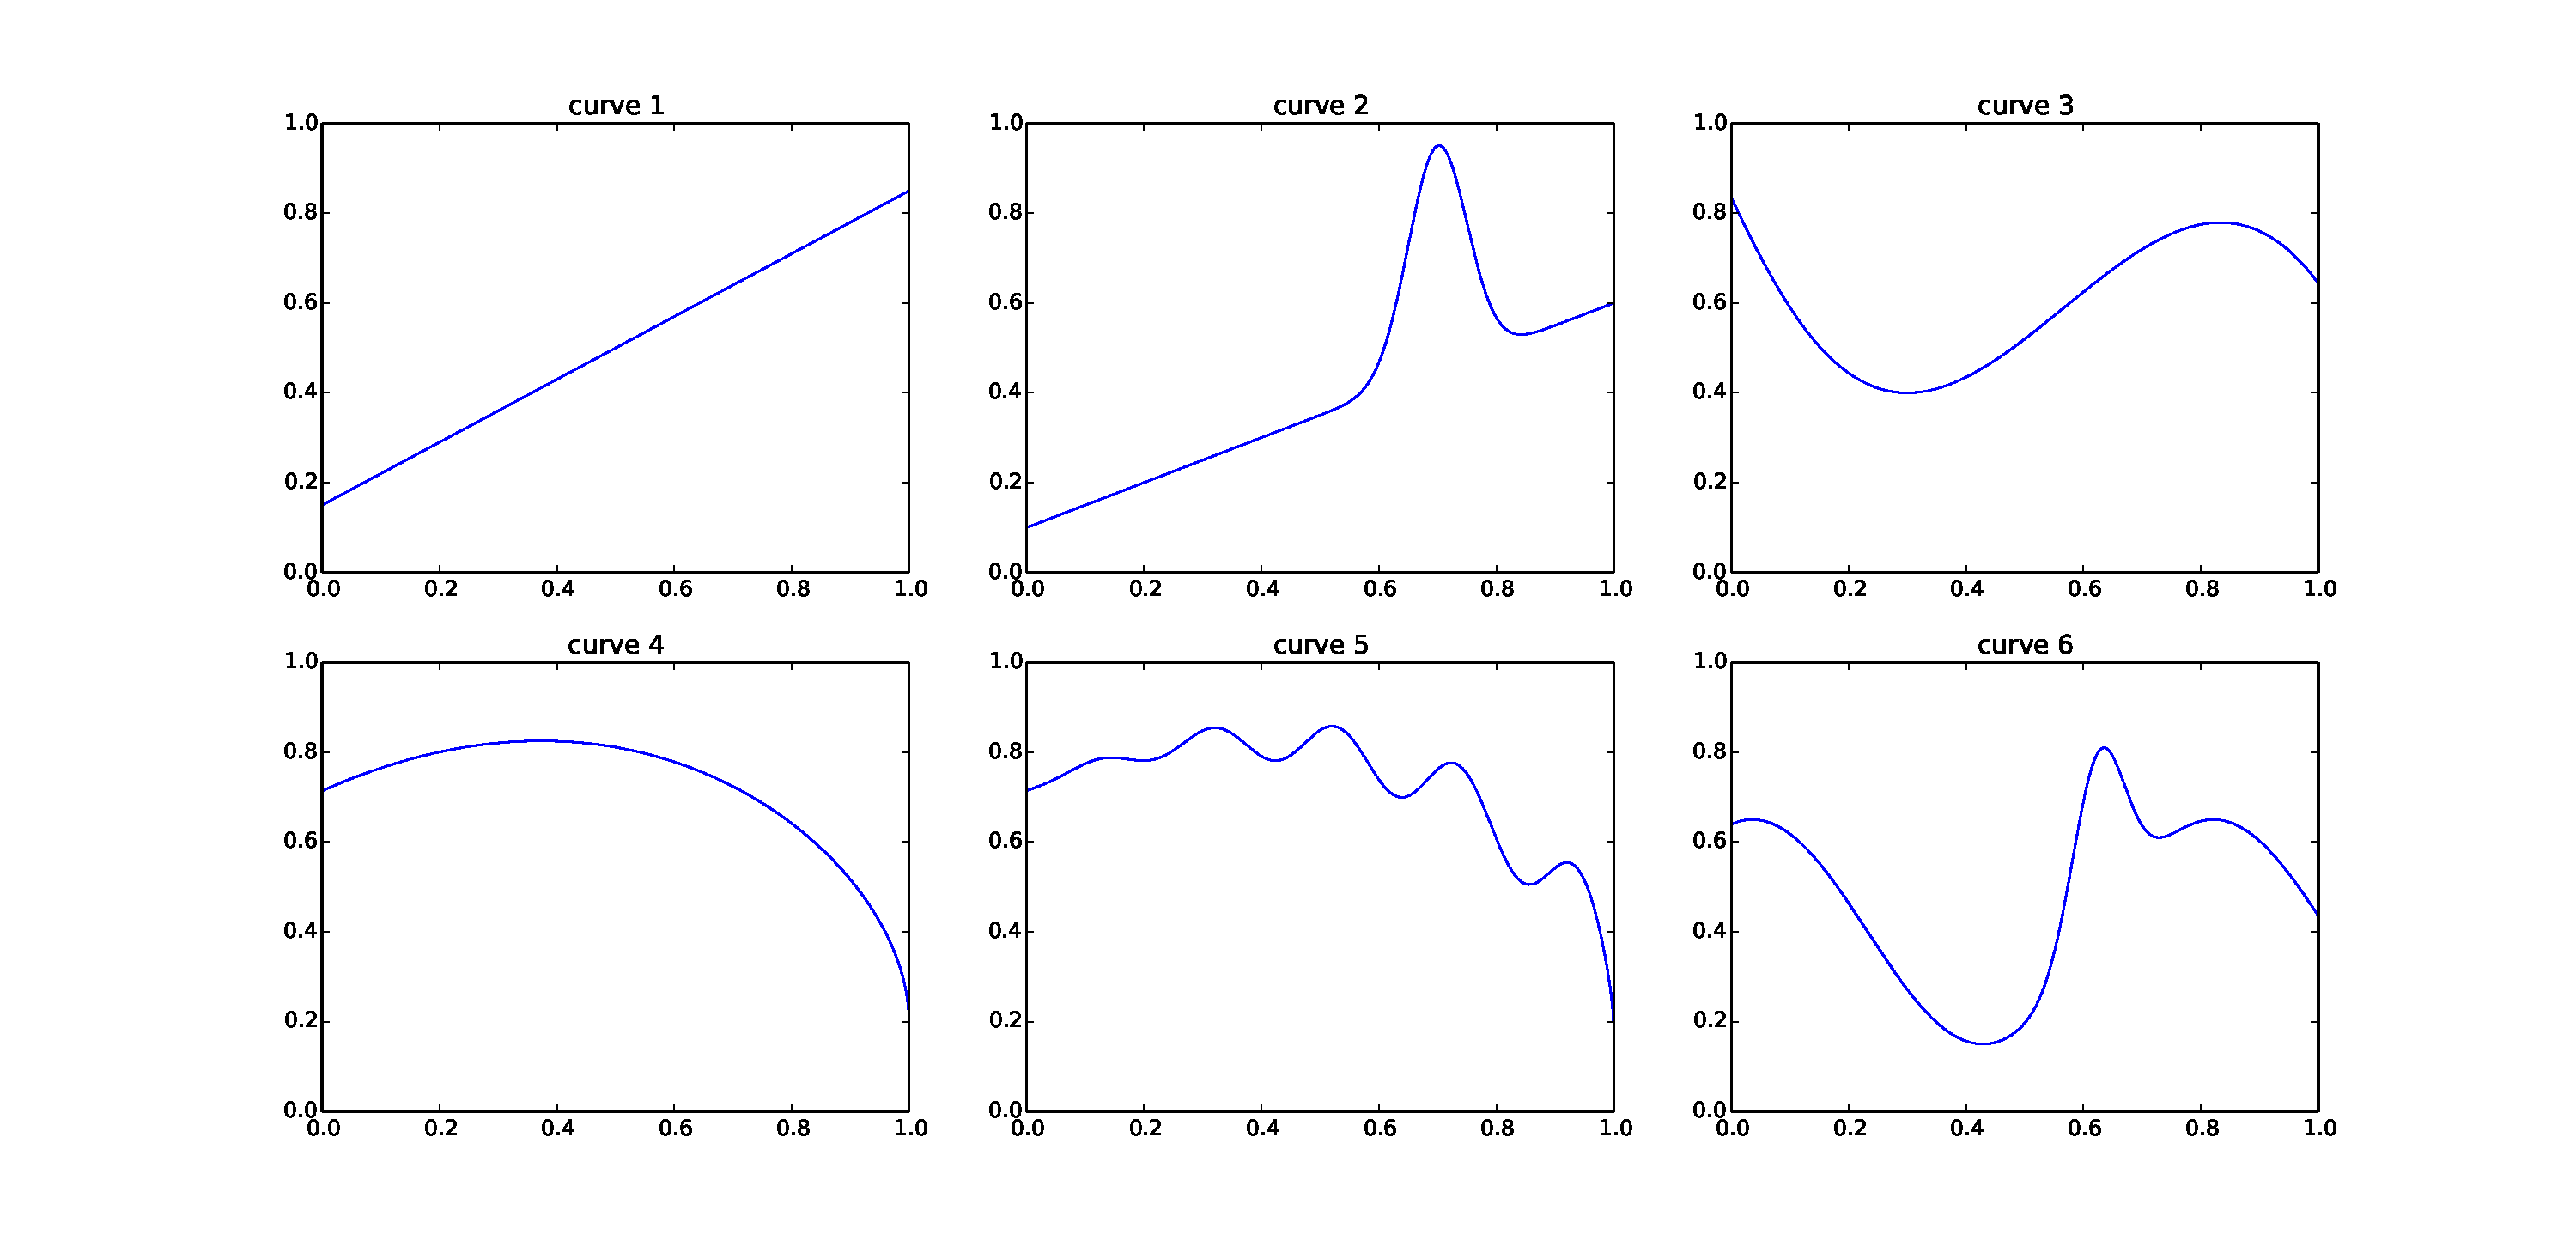
\includegraphics[scale=0.35]{curves}
\end{center}
\vspace{0.5cm}
\caption{Simulation designs for $f_{j}(\cdot)$}\label{t:curves}
\end{table}


\newpage{}

\begin{table}[H]
\vspace{0.5cm}
\begin{tabular}{ccc|cc|cc}
 &  & & \multicolumn{2}{c|}{CI for $W^{*}_{\mathcal{G}}$} & \multicolumn{2}{c}{CS for $G^{*}$}   \tabularnewline
                     &  &            &                  &                 &                           & Average                            \tabularnewline
 Sample                    & Tuning   &            & 90\% CI   & Average   & 90\% CS           & Maximum                          \tabularnewline
 size & parameter & Curve & Coverage & CI length  & Coverage & Regret          \tabularnewline
\hline 
$n=500$& $\epsilon_{n}=n^{-1/6}$ & 1 & 0.882 & 1.780 & 0.944  & -0.767  \tabularnewline
      & & 2 & 0.884 & 1.797 & 0.937  & -0.770   \tabularnewline
     &  & 3 & 0.883 & 1.784 & 0.947  & -0.777  \tabularnewline
     &  & 4 & 0.880 & 1.777 & 0.943  & -0.767  \tabularnewline
     &  & 5 & 0.870 & 1.783 & 0.945  & -0.772  \tabularnewline
     &  & 6 & 0.898 & 1.811 & 0.951  & -0.776  \tabularnewline
\hline 
$n=500$ & $\epsilon_{n}=n^{-1/5}$ & 1 & 0.865 & 1.732 & 0.924 & -0.742  \tabularnewline
      & & 2 & 0.874 & 1.749 & 0.923  & -0.745  \tabularnewline
      & & 3 & 0.871 & 1.737 & 0.927  & -0.753  \tabularnewline
      & & 4 & 0.882 & 1.729 & 0.919  & -0.743  \tabularnewline
     & & 5 & 0.860 & 1.734  & 0.931  & -0.746  \tabularnewline
     & & 6 & 0.882 & 1.762  & 0.929  & -0.751  \tabularnewline
\hline 
$n=500$& $\epsilon_{n}=n^{-1/4}$ & 1 & 0.843 & 1.645 & 0.859 & -0.686  \tabularnewline
     &  & 2 & 0.847 & 1.660 & 0.854  & -0.688  \tabularnewline
    & & 3 & 0.846 & 1.648 & 0.858  & -0.698  \tabularnewline
    &   & 4 & 0.851 & 1.640 & 0.839  & -0.688  \tabularnewline
    &  & 5 & 0.836 & 1.646  & 0.858  & -0.692  \tabularnewline
    &  & 6 & 0.848 & 1.673  & 0.860  & -0.697  \tabularnewline
\hline 
$n=2000$& $\epsilon_{n}=n^{-1/6}$ & 1 & 0.899 & 0.897 & 0.966  & -0.458  \tabularnewline
     &  & 2 & 0.915 & 0.906 & 0.965  & -0.461   \tabularnewline
    & & 3 & 0.927 & 0.902 & 0.962  & -0.458  \tabularnewline
    &   & 4 & 0.912 & 0.899 & 0.970  & -0.458  \tabularnewline
    &   & 5 & 0.913 & 0.903 & 0.968  & -0.464  \tabularnewline
     &  & 6 & 0.928 & 0.918 & 0.971  & -0.463  \tabularnewline
\hline 
$n=2000$ & $\epsilon_{n}=n^{-1/5}$ & 1 & 0.908 & 0.873 & 0.948 & -0.438  \tabularnewline
      & & 2 & 0.903 & 0.880 &  0.946 & -0.442  \tabularnewline
      & & 3 & 0.916 & 0.875 & 0.958  & -0.438  \tabularnewline
      & & 4 & 0.896 & 0.874 & 0.956  & -0.437  \tabularnewline
     & & 5 & 0.903&  0.876 & 0.953 & -0.446  \tabularnewline
     & & 6 & 0.917 & 0.892  & 0.949  & -0.443  \tabularnewline
\hline 
$n=2000$& $\epsilon_{n}=n^{-1/4}$ & 1 & 0.880 & 0.823 & 0.876 & -0.394  \tabularnewline
      & & 2 & 0.881 & 0.829 & 0.880  & -0.398  \tabularnewline
      & & 3 & 0.892 & 0.825 & 0.895 & -0.393  \tabularnewline
      & & 4 & 0.872 & 0.824 & 0.886  & -0.395  \tabularnewline
      & & 5 & 0.876 & 0.826  & 0.883  & -0.399  \tabularnewline
      & & 6 & 0.899 & 0.840  & 0.887  & -0.397  \tabularnewline
\hline 
\hline 
\end{tabular}
\vspace{0.5cm}
\caption{Simulation results}\label{t:sim}
\end{table}

\bibliography{references}
\end{document}
